
\SetKwFunction{FMergeDTs}{MergeDTs}
\SetKwFunction{FDPTimelinesCosts}{DPTimelinesCosts}
\subsection{QPTAS for the $T||V,c||C_{max}$ problem}

The following algorithh is a simplified version of the QPTAS provided in \cite{dereniowski2017ApproxSsForGeneralBSinWTs}. The core idea of the algorithm is the same, however, our solution uses the language of decision trees instead of the language of sequence assignments, which makes the algorithm more intuitive.

For the rest of the analysis, without loss of the generality, we will assume that $T$ is rooted in a vertex $v$ minimizing $c\br{v}$.  We will also assume that all costs are normalized, so that $\max_{v\in V\br{T}}\brc{c\br{v}}=1$. If not, the costs are scaled by dividing them by $\max_{v\in V\br{T}}\brc{c(v)}$. Note that this operation does not affect the optimality of a strategy or the quality of an approximation.
\begin{observation}\label{basicBoundsOnCost}
    Let $T$ be a tree such that $\spr{V\br{T}}> 1$ and $c:V\to \mathbb{R}^+$ be a normalized weight function. Then, $1\leq \OPT(T) \leq \fl{\log n}+1$.
    \begin{proof}
        The first inequality is due to the fact that there exists $v\in V\br{T}$, such that $c\br{v}=1$ and for any decision tree $D$ we have $v\in Q_{D}\br{T,v}$. The second inequality is due to the fact that we can always locate the target using $\fl{\log n}+1$ queries \cite{OnakParys2006GenOfBSSInTsAndFLikePosets}.
    \end{proof}
\end{observation}
\subsubsection{Rounding}
We will use the following rounding schem which will allow us to discretise the space of possible solutions to process it efficiently. Let $p \in\mathbb{N}$, and $k=a/pn$ for some $a\in\mathbb{N}$. Define:
$$
c'\br{v}=\begin{cases}
    \cl{c\br{c}}_k, & \text{if } c\br{v}>pk, \text{ in which case the vertex will be called \textit{heavy}},\\
    \cl{c\br{c}}_{\frac{1}{pn}}, & \text{otherwise, in which case the vertex will be called \textit{light}}.\\
\end{cases}
$$

\begin{lemma}\label{rounded_dt_lemma}
    $$
    \OPT\br{T,c'}\leq \br{1+\frac{2}{p}}\cdot \OPT\br{T,c}
    $$
    \begin{proof}
        Let $D^*$ be an optimal strategy for $\br{T,c}$. By definition, we have that for every vertex $v\in V\br{T}$, $c'\br{v}\leq \br{1+\frac{1}{p}}\cdot c\br{v}+\frac{1}{p}n$ and therefore:
        \begin{align*}
            \OPT\br{T, c'}&\leq \COST_{D^*}\br{T,c'}=\max_{v\in V\br{T}}\brc{\sum_{q\in Q_{D^*}\br{T,v}}c'\br{q}}
            \\&
            \leq \max_{v\in V\br{T}}\brc{\sum_{q\in Q_{D^*}\br{T,v}}\br{\br{1+\frac{1}{p}}\cdot c\br{v}+\frac{1}{pn}}}
            \\&
            \leq \frac{1}{p}+\br{1+\frac{1}{p}}\cdot \max_{v\in V\br{T}}\brc{\sum_{q\in Q_{D^*}\br{T,v}}c\br{v} }\leq \br{1+\frac{2}{p}}\OPT\br{T,c}
        \end{align*}

        where in the third inequality we used the fact that for every $v\in V\br{T}$, $\spr{Q_{D^*}\br{T,v}}\leq n$ and in the last inequality we used Observation \ref{basicBoundsOnCost}.
    \end{proof}
\end{lemma}

While calculating the decision tree, we will divide the time into boxes of duration $k$, which will be further subdivided into $a$ identical slots of length $\frac{1}{pn}$. Let $t_q$ denote the start of some query in a decision tree $D$. Note that the numbers $t_v$ provide a complete information about any decision tree, and are an equiavalent representation of any strategy. We will assume that for any heavy vertex $v\in V\br{T}$, $t_v$ is an integer multiple of $c$ and for any light vertex $v\in V\br{T}$, $t_v$ is an integer multiple of $\frac{1}{pn}$. \footnote{Note that by doing so, we allow decision trees to contain idle time intervals, in which no queries are scheduled. However, if this occurs, after obtaining such decision tree, we simply delete the idle times, which results in a valid decision tree} We have the following lemma:
\begin{lemma}\label{aligned_dts_lemma}
    There exists a decision tree $D$ for $\br{T,c'}$, such that $\COST_{D}\br{T, c'}\leq \br{1+\frac{3}{p}}\cdot\OPT\br{T, c'}$ and for every vertex $v\in V\br{T}$ we have:
    \begin{enumerate}
        \item if $c\br{v}> pk$, then $t_v/k\in\mathbb{N}$ (every heavy query is aligned to a multiple of $c$),
        \item if $c\br{v}\leq pk$, then $t_vpn\in\mathbb{N}$ (every light query is aligned to a multiple of $\frac{1}{pn}$).
    \end{enumerate}
    \begin{proof}
        Let $D^*$ by any optimal decision tree for $\br{T,c'}$. For any $v\in V\br{T}$, let $t_v^*$ be the start of query to $v$ in $D^*$ and let $t_v'=\br{1+\frac{2}{p}}t_v^*$, thus construction a new decision tree $D'$. Since in this new decision tree $D'$, the ordering of vertices is exactly the same as in $D^*$, for any two consecutive queries $v,u$ in $D'$ we have:
        $$
            t_u'-t_v'=\br{1+\frac{2}{p}}\cdot\br{t_u-t_v}\geq \br{1+\frac{2}{p}}\cdot c\br{v}
        $$

        We now construct $D$ as follows: If $v\in V\br{T}$ is heavy, we assign $t_v=\cl{t_v'}_k$ and $t_v=t_v'$ otherwise. For any two consecutive queries $v,u$ in $D$, such that $v$ is heavy we have:
        $$
        t_u-\cl{t_v'}_k>t_u-t_v-k\geq \br{1+\frac{2}{p}}\cdot c\br{v}-k>w\br{v}+k>c'\br{v}
        $$

        So we conclude that no two queries overlap. To obtain the second part of the claim, we round up the starting time of each query to a light vertex in $D$ to an integer multiple of $\frac{1}{pn}$. We have:
        \begin{align*}
            \COST_{D}\br{T,c'}&
            \leq \max_{v\in V\br{T}}\brc{\sum_{q\in Q_{D^*}\br{T,v}}\br{\br{1+\frac{2}{p}}\cdot c'\br{v}+\frac{1}{pn}}}
            \\&
            \leq \frac{1}{p}+\br{1+\frac{2}{p}}\cdot \max_{v\in V\br{T}}\brc{\sum_{q\in Q_{D^*}\br{T,v}}c'\br{v} }\leq \br{1+\frac{3}{p}}\OPT\br{T,c'}
        \end{align*}

        where in the third inequality we used the fact that for every $v\in V\br{T}$, $\spr{Q_{D}\br{T,v}}\leq n$ and in the last inequality we used Observation \ref{basicBoundsOnCost}.
    \end{proof}
\end{lemma}

We will call a decision tree fulfilling above conditions \textit{aligned}. In subsequent considerations, we will focus ourselves of finding such decision trees, whose properties will allow us to devise an efficient dynamic programming procedure finding an optimal, aligned decision tree. 

\subsubsection{Heavy module contraction, up and down responses}
Since, our decision tree is rooted, we can reasonably talk about up and down responses to a query. An \textit{up} response to a query to $v$ in $T$ occurs when the connected component $\in T-v$, which is the reply happens to contain $r\br{T}$. If this is not the case, then such response is called a \textit{down} response. As it will turns out, a repeating occurance of light queries with down responses will become problematic for our algorithm. To account for this issue we will use the following notions:

We will define a new measure of cost for aligned decision trees called the \textit{aligned cost}. Let $D$ be any aligned strategy for $\br{t,c'}$. For any  vertex $v\in V\br{T}$ and query $q\in Q_{D}\br{T,v}$ the contribution $\kappa_{T,c,k}\br{q,v}$ of $u$ is defined as:
$$
\kappa_{T,c}\br{q, v}= \begin{cases}
    \fl{t_v+c\br{q}}_k-t_v, & \text{if } c\br{v}\leq pk \text{ and the response to query $q$ in $T$, towards $v$ is down},\\
    c\br{q}, & \text{otherwise}.
\end{cases}
$$

Then, the \textit{aligned cost} of $D$ is defined as:

$$
\COST'_D\br{T,c',k}=\max_{v\in V\br{T}}\brc{\sum_{q\in Q_D\br{T,v}}\kappa_{T,c', k}\br{q,v}}.
$$

Let $\OPT'\br{T,c',k}$ denote the optimal aligned cost among all aligned decision trees for $\br{T,c',k}$.
Notice that in the above cost, we lose $k$ query time per light query with a down response. Since of course, the amount of such queries may be of order $O\br{n}$, the difference between $\COST'_D\br{T,c',k}$ and $\COST_D\br{T,c',k}$ may grow almost arbitrarily large. However, we will make sure that this does not happen to often, which will give us the desired bound on the cost of the solution. We have the following simple observation:
\begin{observation}\label{aligned_subtree_opt_observation}
    Let $T'$ be a subtree of $T$. Then, $\OPT'\br{T'}\leq\OPT'\br{T}$.
\end{observation}


\begin{figure}[htbp]
    \begin{minipage}[t]{0.5\textwidth}
    \centering
    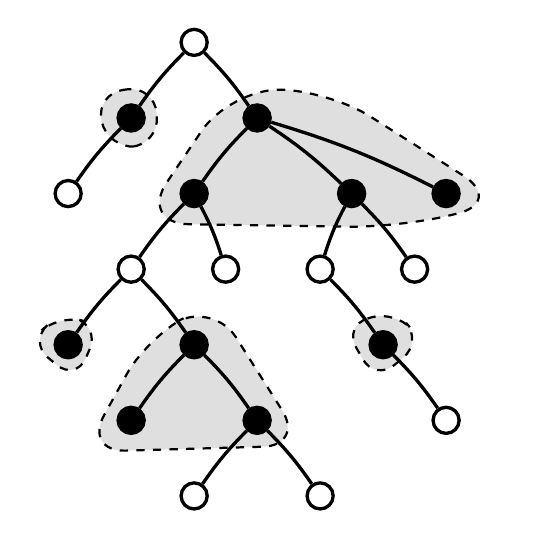
\begin{tikzpicture}[every node/.style={draw, very thick}, every path/.style={very thick}]
    
    \draw[dashed, thick, rounded corners = 10pt, fill= gray!25]
         (-1.25,5.75)  -- (-0.5,5.85)--  (-0.45,5.1) -- (-1.1,5.05) -- cycle;

    \draw[dashed, thick, rounded corners = 18pt, fill= gray!25]
        (0.45,5.8)  -- (1.7,5.8)-- (3.95,4.37) -- (2.6,4.05) -- (-0.7,4.1) -- cycle;
    \draw[dashed, thick, rounded corners = 9pt, fill= gray!25]
        (-2.1,2.6) -- (-1.7,2.95) -- (-1.2,2.8)  -- (-1.5,2.1) -- cycle;
        
    \draw[dashed, thick, rounded corners = 15pt, fill= gray!25]
         (-0.6,2.65) -- (0.25,3.1) -- (1.4,1.28) -- (-1.4,1.2) -- cycle;

    \draw[dashed, thick, rounded corners = 9pt, fill= gray!25]
        (1.9,2.8)  -- (2.55,3)  -- (2.9,2.6) -- (2.3,2.1) -- cycle;
    
    \node[circle, draw, fill=white] (1) at (0,6.4) {};
    
    \node[circle, draw, fill=black] (2) at (-0.8,5.44) {};
    \node[circle, draw, fill=black] (3) at (0.8,5.44) {};

    \node[circle, draw, fill=white] (4) at (-1.6,4.48) {};
    \node[circle, draw, fill=black] (5) at (0,4.48) {};
    \node[circle, draw, fill=black] (6) at (2.0,4.48) {};
    \node[circle, draw, fill=black] (7) at (3.2,4.48) {};
    
    \node[circle, draw, fill=white] (8) at (-0.8,3.52) {};
    \node[circle, draw, fill=white] (9) at (0.4,3.52) {};
    \node[circle, draw, fill=white] (10) at (1.6,3.52) {};
    \node[circle, draw, fill=white] (11) at (2.8,3.52) {};
    
    \node[circle, draw, fill=black] (12) at (-1.6,2.56) {};
    \node[circle, draw, fill=black] (13) at (0,2.56) {};
    \node[circle, draw, fill=black] (14) at (2.4,2.56) {};
    
    \node[circle, draw, fill=black] (15) at (-0.8,1.6) {};
    \node[circle, draw, fill=black] (16) at (0.8,1.6) {};
    \node[circle, draw, fill=white] (17) at (3.2,1.6) {};
    
    \node[circle, draw, fill=white] (18) at (0,0.64) {};
    \node[circle, draw, fill=white] (19) at (1.6,0.64) {};
    
    \draw[bend right=5] (1) to (2);
    \draw[bend left=5] (1) to (3);
    
    \draw[bend right=5] (2) to (4);
    \draw[bend right=5] (3) to (5);
    \draw[bend left=5] (3) to (6);
    \draw[bend left=5] (3) to (7);
    
    \draw[bend right=5] (5) to (8);
    \draw[bend left=5] (5) to (9);
    \draw[bend right=5] (6) to (10);
    \draw[bend left=5] (6) to (11);
    
    \draw[bend right=5] (8) to (12);
    \draw[bend left=5] (8) to (13);
    \draw[bend left=5] (10) to (14);
    
    \draw[bend right=5] (13) to (15);
    \draw[bend left=5] (13) to (16);
    \draw[bend left=5] (14) to (17);
    
    \draw[bend right=5] (16) to (18);
    \draw[bend left=5] (16) to (19);

    \end{tikzpicture}
\end{minipage}
    \begin{minipage}[t]{0.5\textwidth}
    \centering
    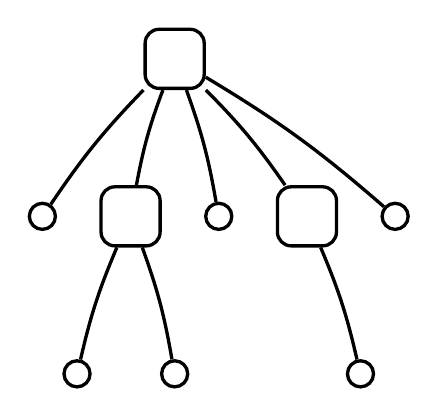
\begin{tikzpicture}[every node/.style={draw,rounded corners=5pt, very thick}, every path/.style={very thick}]
    
    \node[rectangle, minimum size=0.75cm, draw] (1) at (-0.56,10) {};
    
    \node[circle, draw] (2) at (-2.24,8) {};
    \node[rectangle, minimum size=0.75cm, draw] (3) at (-1.12,8) {};
    \node[circle, draw] (4) at (0,8) {};
    \node[rectangle, minimum size=0.75cm, draw] (5) at (1.12,8) {};
    \node[circle, draw] (6) at (2.24,8) {};
    
    \node[circle, draw] (7) at (-1.8,6) {};
    \node[circle, draw] (8) at (-0.56,6) {};
    \node[circle, draw] (9) at (1.8,6) {};
    
    \draw[bend right=5] (1) to (2);
    \draw[bend right=5] (1) to (3);
    \draw[bend left=5] (1) to (4);
    \draw[bend left=5] (1) to (5);
    \draw[bend left=5] (1) to (6);
    
    \draw[bend right=5] (3) to (7);
    \draw[bend left=5] (3) to (8);
    \draw[bend left=5] (5) to (9);

    \end{tikzpicture}
\end{minipage}
    \caption[Heavy module contraction]{Example of contracting 5 heavy modules. Black vertices represent heavy vertices, white vertices represent light vertices and square vertices represent vertices which were a parent of at least one heavy module before contraction.}\label{exampleHeavymoduleContraction}
\end{figure}
We define a \textit{heavy module} as $H\subseteq V\br{T}$ such that: $T[H]$ is connected, every $v \in H$ is heavy, i. e., $c\br{v}\geq pk$ and $H$ is maximal - no vertex can be added to it without violating one of its properties. A \textit{contraction} of a heavy module $H$ is an operation which consists of deleting all of the vertices in $H$ from $T$ and connecting every vertex $u$ which was a child of some vertex in $H$ to the parent of $r\br{T\angl{H}}$ if it exists. For example see Figure \ref{exampleHeavymoduleContraction}.

\subsubsection{The main procedure}

We will use the following propositions:
\begin{proposition}\label{DPTimelinesCostsProposition}
     Let $T$ be a tree, $c'$ an aligned cost function, $p\in \mathbb{N}$, $k$ the box size and $d\in \mathbb{N}$~be the depth. There exists a \FDPTimelinesCosts procedure, which (if it exists) calculates an aligned decision tree $D$ for $\br{T,c'}$ of cost at most $\COST'_D\br{T,c',k}\leq kd$, running in $\br{pn}^{O\br{d}}$ time.
\end{proposition}
\begin{proposition}\label{MergeDTsProposition}
    Let $T$ be a tree, $c'$ be an aligned cost function, $p\in \mathbb{N}$, $k\in \mathbb{R}_{>0}$ be the box size, $D_A$ be a decision tree for $T$ and $F_C$ be forest of decision trees for $T$ with all heavy modules contracted. There exists a polynomial time \FMergeDTs procedure which returns a decision tree of cost at most:
        $$
            \COST_{D}\br{T,c',k}\leq\COST'_{D_A}\br{T,c',k}+2pk\cdot \COST_{F_C}\br{T,1}.
        $$
\end{proposition}
The proofs will be provided in the further sections.
We will now prove the Proposition \ref{QPTAS}.


\begin{algorithm}
\caption{The QPTAS for $T||V,c,w||C_{max}$.}\label{qptas_pseudocode}
\SetKwProg{Fn}{Procedure}{:}{}
\Fn{$\FQPTAS\br{T,c,\epsilon}$}{
    $p\gets\cl{24/\epsilon}$,
    $k\gets 0$,
    $D\gets \emptyset$.

    $d\gets p^2\cdot\br{\fl{\log\br{n}}+1}$.

    \Repeat{$D \neq \emptyset$}
    {
        $k\gets k+\frac{1}{pn}$.

        \ForEach{$v\in V\br{T}$}{
            \If{$c\br{v}>pk$}{
                $c'\br{v}\gets \cl{c\br{v}}_k$.
            }
            \Else{
                $c'\br{v}\gets \cl{c\br{v}}_{\frac{1}{pn}}$.
            }
            
        }

        $T_C\gets T$ with all heavy modules contracted.

        $D_C\gets\FRankingBasedDT\br{T_C}$.

        $D\gets \FBuildDT\br{T, c', D_C, p, k, d}$.
    }   
    \Return $D$.
    
}
\end{algorithm}

The Algorithm \ref{qptas_pseudocode} starts by picking $p=\cl{\frac{59}{\epsilon}}$, $d=p^2\cdot\br{\fl{\log n}+1}$ and $k=0$ and. At each iteration of the repeat loop, the algorithm picks $k$ to be the next 
integer multiple of $\frac{1}{pn}$ and performs the rounding operation. After that, the Proposition \label{DPTimelinesCostsProposition} is applied for $\br{T,c',p,k,d}$. If the returned decision tree $D_A\neq\emptyset$, then a new tree $T_C$ is constructed by contracting all heavy modules of $T$. By calling the \FRankingBasedDT for $T_C$, the algorithm builds a second decision tree $D_C$, and then merges it with $D_A$ by applying Proposition \label{MergeDTsProposition}. Then, the algorithm returns the resulting decision $D$.

Let $k'$ be the value of $k$ for which $D$ was built. Let $k''=k-\frac{1}{pn}$ and $c''$ be the values of $k$ and $c'$ of the previous iteration of the while loop. Since we know that for $k''$ and $c''$ we had $D_A=\emptyset$, by Proposition \ref{DPTimelinesCostsProposition} we have that $k'' d \leq \OPT'\br{T,c''}$. Hence,
 $k'\leq \frac{\OPT'\br{T,c'',k'}}{d}+\frac{1}{pn}\leq\frac{2\cdot \OPT'\br{T,c'',k''}}{p^2\cdot\br{\fl{\log n}+1}}$, so we have that:
\begin{align*}
    \COST_{D}\br{T,c'}&\leq \OPT'\br{T,c',k'}+2pk'\cdot \br{\fl{\log n}+1}
    \\&\leq \OPT'\br{T,c'',k''}+2p\cdot \br{\fl{\log n}+1}\cdot \frac{2\cdot\OPT'\br{T,c'', k''}}{p^2\cdot\br{\fl{\log n}+1}} \\
    & \leq \br{1+\frac{4}{p}}\cdot\OPT'\br{T,c'',k''}\leq \br{1+\frac{2}{p}}\cdot\br{1+\frac{3}{p}}\cdot\br{1+\frac{4}{p}}\cdot\OPT\br{T,c}
    \\&
    \leq \br{1+\frac{59}{p}}\cdot\OPT\br{T,c} = \br{1+\frac{59}{\cl{\frac{59}{\epsilon}}}}\cdot\OPT\br{T,c}\leq \br{1+\epsilon}\cdot \OPT\br{T,c}
\end{align*}
    
where the first inequality is by Proposition \ref{MergeDTsProposition}, the second inequality is by the fact that $\OPT\br{T,c',k'}\leq \OPT\br{T,c',k''}$ and by applying Corollary \ref{vertexRankingCorollary} and the fourth inequality is by the fact that $\OPT\br{T,c',k''}\leq \OPT\br{T,c}$, Lemma \ref{rounded_dt_lemma} and Lemma \ref{aligned_dts_lemma}.

We can assume that $c=\text{poly}\br{n}$, since beyond that the problem can be solved to optimality in $O\br{2^nn}$ time. Therefore the running time of the procedure is bounded by:
$$
n^{O\br{d}}=n^{O\br{p^2\log n}}=n^{O\br{\log n/\epsilon^2}}.
$$
\subsubsection{Proof of Proposition \ref{MergeDTsProposition}}


\begin{algorithm}
\caption{The \FMergeDTs procedure.}\label{mergeDTspseudocode}
\SetKwProg{Fn}{Procedure}{:}{}
\Fn{$\FMergeDTs\br{T, D_A, F_C}$}{
    \If{$F_C$ is connected}{
        $r\gets r\br{F_C}$.
    }
    \Else{
        $r\gets r\br{D_A}$.
    }
    $D\gets \br{\brc{r}, \emptyset}$.
    \ForEach{$T'\in T-r$}{
        $D'\gets \FMergeDTs\br{T, D_A|T', F_C|T'}$.

        Hang $D'$ below $r$ in $D$.
    }
    \Return $D$.
}
\end{algorithm}
% 
\SetKwFunction{FDPTimelines}{DPTimelines}
\begin{figure}[htp]
\begin{minipage}[t]{1\textwidth}
    \centering
    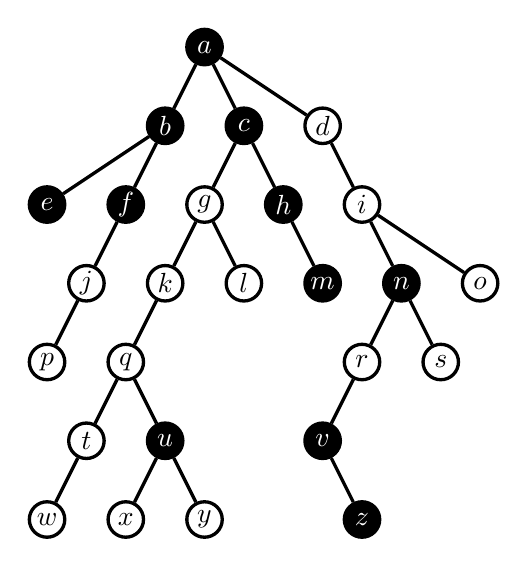
\begin{tikzpicture}[every path/.style={very thick}]
    
    \node[text=white, circle, draw, minimum size=0.45cm, inner sep=0pt, fill=black] (1) at (0,0) {$a$};

    \node[text=white, circle, draw, minimum size=0.45cm, inner sep=0pt, fill=black] (2) at (-0.5,-1) {$b$};

    \node[text=white, circle, draw, minimum size=0.45cm, inner sep=0pt, fill=black] (3) at (0.5,-1) {$c$};

    \node[circle, draw, minimum size=0.45cm, inner sep=0pt, fill=white] (4) at (1.5,-1) {$d$};

    \draw[] (1) to (2);
    \draw[] (1) to (3);
    \draw[] (1) to (4);

    \node[text=white, circle, draw, minimum size=0.45cm, inner sep=0pt, fill=black] (5) at (-2,-2) {$e$};

    \node[text=white, circle, draw, minimum size=0.45cm, inner sep=0pt, fill=black] (6) at (-1,-2) {$f$};

    \node[circle, draw, minimum size=0.45cm, inner sep=0pt, fill=white] (7) at (0,-2) {$g$};

    \node[text=white, circle, draw, minimum size=0.45cm, inner sep=0pt, fill=black] (8) at (1,-2) {$h$};

    \node[circle, draw, minimum size=0.45cm, inner sep=0pt, fill=white] (9) at (2,-2) {$i$};

    \draw[] (2) to (5);
    \draw[] (2) to (6);

    \draw[] (3) to (7);
    \draw[] (3) to (8);

    \draw[] (4) to (9);

    \node[circle, draw, minimum size=0.45cm, inner sep=0pt, fill=white] (10) at (-1.5,-3) {$j$};

    \node[circle, draw, minimum size=0.45cm, inner sep=0pt, fill=white] (11) at (-0.5,-3) {$k$};

    \node[circle, draw, minimum size=0.45cm, inner sep=0pt, fill=white] (12) at (0.5,-3) {$l$};

    \node[text=white, circle, draw, minimum size=0.45cm, inner sep=0pt, fill=black] (13) at (1.5,-3) {$m$};

    \node[text=white, circle, draw, minimum size=0.45cm, inner sep=0pt, fill=black] (14) at (2.5,-3) {$n$};

    \node[circle, draw, minimum size=0.45cm, inner sep=0pt, fill=white] (15) at (3.5,-3) {$o$};

    \draw[] (6) to (10);

    \draw[] (7) to (11);
    \draw[] (7) to (12);

    \draw[] (8) to (13);

    \draw[] (9) to (14);
    \draw[] (9) to (15);

    \node[circle, draw, minimum size=0.45cm, inner sep=0pt, fill=white] (16) at (-2,-4) {$p$};

    \node[circle, draw, minimum size=0.45cm, inner sep=0pt, fill=white] (17) at (-1,-4) {$q$};

    \node[circle, draw, minimum size=0.45cm, inner sep=0pt, fill=white] (18) at (2,-4) {$r$};

    \node[circle, draw, minimum size=0.45cm, inner sep=0pt, fill=white] (19) at (3,-4) {$s$};

    \draw[] (10) to (16);
    
    \draw[] (11) to (17);
    
    \draw[] (14) to (18);
    \draw[] (14) to (19);

    \node[circle, draw, minimum size=0.45cm, inner sep=0pt, fill=white] (20) at (-1.5,-5) {$t$};

    \node[text=white, circle, draw, minimum size=0.45cm, inner sep=0pt, fill=black] (21) at (-0.5,-5) {$u$};

    \node[text=white, circle, draw, minimum size=0.45cm, inner sep=0pt, fill=black] (22) at (1.5,-5) {$v$};

    \draw[] (17) to (20);
    \draw[] (17) to (21);

    \draw[] (18) to (22);


    \node[circle, draw, minimum size=0.45cm, inner sep=0pt, fill=white] (23) at (-2,-6) {$w$};

    \node[circle, draw, minimum size=0.45cm, inner sep=0pt, fill=white] (24) at (-1,-6) {$x$};

    \node[circle, draw, minimum size=0.45cm, inner sep=0pt, fill=white] (25) at (0,-6) {$y$};

    \node[text=white, circle, draw, minimum size=0.45cm, inner sep=0pt, fill=black] (26) at (2,-6) {$z$};

    
    \draw[] (20) to (23);

    \draw[] (21) to (24);
    \draw[] (21) to (25);

    \draw[] (22) to (26);
    
    \end{tikzpicture}
    \caption[Input tree $T$ with a heavy root]{}\label{tree_h_root}
\end{minipage}
\begin{minipage}[t]{0.49\textwidth}
    \centering
    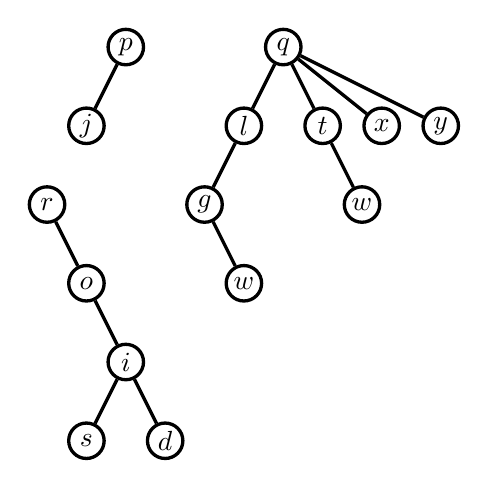
\begin{tikzpicture}[every path/.style={very thick}]
    
    \node[circle, draw, minimum size=0.45cm, inner sep=0pt, fill=white] (1) at (0,0) {$p$};

    \node[circle, draw, minimum size=0.45cm, inner sep=0pt, fill=white] (2) at (-0.5,-1) {$j$};

    \draw[] (1) to (2);

    \node[circle, draw, minimum size=0.45cm, inner sep=0pt, fill=white] (3) at (2,0) {$q$};



    \node[circle, draw, minimum size=0.45cm, inner sep=0pt, fill=white] (4) at (1.5,-1) {$l$};

    \node[circle, draw, minimum size=0.45cm, inner sep=0pt, fill=white] (5) at (2.5,-1) {$t$};

    \node[circle, draw, minimum size=0.45cm, inner sep=0pt, fill=white] (6) at (3.25,-1) {$x$};

    \node[circle, draw, minimum size=0.45cm, inner sep=0pt, fill=white] (7) at (4,-1) {$y$};

    

    \draw[] (3) to (4);
    \draw[] (3) to (5);
    \draw[] (3) to (6);
    \draw[] (3) to (7);

    \node[circle, draw, minimum size=0.45cm, inner sep=0pt, fill=white] (8) at (1,-2) {$g$};

    \node[circle, draw, minimum size=0.45cm, inner sep=0pt, fill=white] (9) at (3,-2) {$w$};

    \draw[] (4) to (8);
    \draw[] (5) to (9);

    \node[circle, draw, minimum size=0.45cm, inner sep=0pt, fill=white] (10) at (1.5,-3) {$w$};

    \draw[] (8) to (10);



    \node[circle, draw, minimum size=0.45cm, inner sep=0pt, fill=white] (11) at (-1,-2) {$r$};


    \node[circle, draw, minimum size=0.45cm, inner sep=0pt, fill=white] (12) at (-0.5,-3) {$o$};

    \draw[] (11) to (12);

    \node[circle, draw, minimum size=0.45cm, inner sep=0pt, fill=white] (13) at (0,-4) {$i$};

    \draw[] (12) to (13);

    \node[circle, draw, minimum size=0.45cm, inner sep=0pt, fill=white] (14) at (-0.5,-5) {$s$};

    \node[circle, draw, minimum size=0.45cm, inner sep=0pt, fill=white] (15) at (0.5,-5) {$d$};

    \draw[] (13) to (14);
    \draw[] (13) to (15);


    
    \end{tikzpicture}
    \caption[Input forest of decision trees for light vertices $F_C$.]{}\label{input_forest}
\end{minipage}
\begin{minipage}[t]{0.49\textwidth}
    \centering
    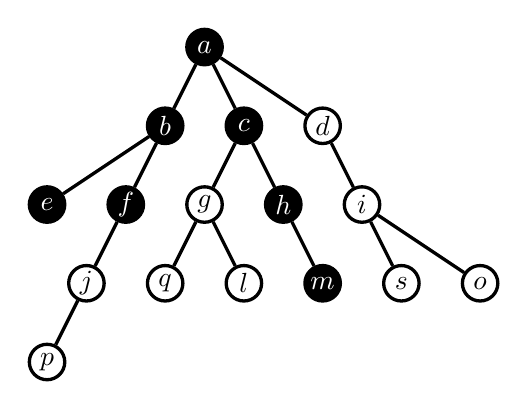
\begin{tikzpicture}[every path/.style={very thick}]
    
    \node[text=white, circle, draw, minimum size=0.45cm, inner sep=0pt, fill=black] (1) at (0,0) {$a$};

    \node[text=white, circle, draw, minimum size=0.45cm, inner sep=0pt, fill=black] (2) at (-0.5,-1) {$b$};

    \node[text=white, circle, draw, minimum size=0.45cm, inner sep=0pt, fill=black] (3) at (0.5,-1) {$c$};

    \node[circle, draw, minimum size=0.45cm, inner sep=0pt, fill=white] (4) at (1.5,-1) {$d$};

    \draw[] (1) to (2);
    \draw[] (1) to (3);
    \draw[] (1) to (4);

    \node[text=white, circle, draw, minimum size=0.45cm, inner sep=0pt, fill=black] (5) at (-2,-2) {$e$};

    \node[text=white, circle, draw, minimum size=0.45cm, inner sep=0pt, fill=black] (6) at (-1,-2) {$f$};

    \node[circle, draw, minimum size=0.45cm, inner sep=0pt, fill=white] (7) at (0,-2) {$g$};

    \node[text=white, circle, draw, minimum size=0.45cm, inner sep=0pt, fill=black] (8) at (1,-2) {$h$};

    \node[circle, draw, minimum size=0.45cm, inner sep=0pt, fill=white] (9) at (2,-2) {$i$};

    \draw[] (2) to (5);
    \draw[] (2) to (6);

    \draw[] (3) to (7);
    \draw[] (3) to (8);

    \draw[] (4) to (9);

    \node[circle, draw, minimum size=0.45cm, inner sep=0pt, fill=white] (10) at (-1.5,-3) {$j$};

    \node[circle, draw, minimum size=0.45cm, inner sep=0pt, fill=white] (11) at (-0.5,-3) {$q$};

    \node[circle, draw, minimum size=0.45cm, inner sep=0pt, fill=white] (12) at (0.5,-3) {$l$};

    \node[text=white, circle, draw, minimum size=0.45cm, inner sep=0pt, fill=black] (13) at (1.5,-3) {$m$};

    \node[circle, draw, minimum size=0.45cm, inner sep=0pt, fill=white] (14) at (2.5,-3) {$s$};

    \node[circle, draw, minimum size=0.45cm, inner sep=0pt, fill=white] (15) at (3.5,-3) {$o$};

    \draw[] (6) to (10);

    \draw[] (7) to (11);
    \draw[] (7) to (12);

    \draw[] (8) to (13);

    \draw[] (9) to (14);
    \draw[] (9) to (15);

    \node[circle, draw, minimum size=0.45cm, inner sep=0pt, fill=white] (16) at (-2,-4) {$p$};


    \draw[] (10) to (16);

    
    \end{tikzpicture}
    \caption[Medusa tree $T_M$]{}\label{medusa_tree}
\end{minipage}
\caption[Construction of the medusa tree]{Construction of the medusa tree. Figure \ref{tree_h_root} shows example input tree $T$ with a heavy root. Figure \ref{input_forest} shows example input forest of decision trees for light vertices $F_C$. Figure \ref{medusa_tree} shows the constructed medusa tree $T_M$.}\label{medusa_tree_construction_figure}
\end{figure}

The algorithm \ref{mergeDTspseudocode} takes as arguments a tree $T$, a decision tree $D_A$ and a forest of decision trees $F_C$ for $T$ with heavy groups contracted. Since $F_C$ may not be a valid partial decision tree for $T_$, it may happen that it is disconnected. This because, after performing a light query to $v$ according to $F_C$, if the response was down and $v$ has heavy child modules, the children of $v$ in $T_C$, may not be separated yet. Based on this, we derive two cases for our procedure:
\begin{enumerate}
    \item $F_C$ is connected. In such case we pick $r=r\br{F_C}$. 
    \item $F_C$ is disconnected. In such case we pick $r=r\br{D_A}$.
\end{enumerate}
We set $D=\br{\brc{r}, \emptyset}$ and then, for each $T'\in T-r$,  we build a decision tree $D'$ for $T'$ recursively by calling \FMergeDTs with arguments $\br{T, D_A|T', F_C|T'}$ and hang $D'$ below $r$ in $D$.
\begin{lemma}
Let $D$ be the decision tree returned by the \FMergeDTs procedure. Then, $
            \COST_{D}\br{T,c',k}\leq\COST'_{D_A}\br{T,c',k}+2pk\cdot \COST_{F_C}\br{T,1}.
        $
\begin{proof}
     Let $x\in V\br{T}$. We have two cases:
    \begin{enumerate}
        \item $r$ is heavy or $r$ is light and the response is up. In this case the cost of query to $r$ is incorporated into $\COST'_{D_A}\br{T,c',k}$.
        \item $r$ is light and the response is down. Let  $r_1$ and $r_2$ be two consecutive light queries in $Q_D\br{T,x}$ with a down response, and let $T''\in T-\brc{r_1, r_2}$, such that $x\in T''$. We will show that $\COST_{F_C|T}\br{T,1}\leq \COST_{F_C}\br{T,1}-1$, so the additional cost of such queries is at most $2pk\cdot \COST_{F_C}\br{T,1}$.
        \begin{enumerate}
            \item $F_C$ is connected. In such case $r_1=r\br{F_C}$ so after query to $r_1$, by definition of the decision tree $\COST_{F_C|T'}\br{T,1}\leq \COST_{F_C}\br{T,1}-1$.
            
            \item $F_C$ is disconnected. Let $T'$ be any down response to query to $r$. If $r_1=r\br{F_C|T'}$, then $\COST_{F_C|T'}\br{T',1}\leq \COST_{F_C}\br{T,1} - 1$. Otherwise, we argue that $F_C|T'$ is connected. Assume contrary. Firstly, we observe that $F_{C}|T_{r_1}$ is connected. This is because, $r_1$ is light, so the tree $T_{r_1,C}$ denoting $T_{r_1}$ with all heavy modules contracted is connected. By assumption, there at least two connected components $D_1,D_2,\dots,D_j$ of $F_C|T'$, with roots $d_1,d_2,\dots, d_j$ respectively. Since every other query $q\in V\br{F_C|T'}$ is a descendant of some $d_1,\dots,d_j$, the only query which could be the parent of $d_1,\dots, d_j$ in $F_C|T'$ is $r_1$, which is a contradiction. Therefore, the next query $r_2$ of $D$ in $T'$ is $r\br{F_C|T'}$. We get that by definition of the decision tree $\COST_{F_C|T''}\br{T,1}\leq \COST_{F_C}\br{T,1}-1$.
        \end{enumerate} 
    \end{enumerate}
\end{proof}
\end{lemma}


\subsubsection{Dynamic programming procedure for a fixed box size}


\SetKwFunction{FDPTimelines}{DPTimelines}
\begin{figure}[htp]
\begin{minipage}[t]{0.49\textwidth}
    \centering
    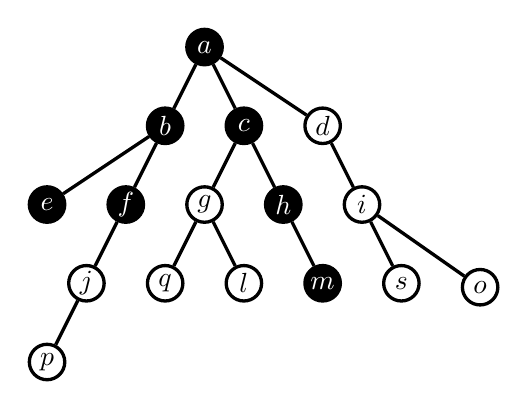
\begin{tikzpicture}[every path/.style={very thick}]

    \node[text=white, circle, draw, minimum size=0.45cm, inner sep=0pt, fill=black] (1) at (0,0) {$a$};

    \node[text=white, circle, draw, minimum size=0.45cm, inner sep=0pt, fill=black] (2) at (-0.5,-1) {$b$};

    \node[text=white, circle, draw, minimum size=0.45cm, inner sep=0pt, fill=black] (3) at (0.5,-1) {$c$};

    \node[circle, draw, minimum size=0.45cm, inner sep=0pt] (4) at (1.5,-1) {$d$};

    \draw[] (1) to (2);
    \draw[] (1) to (3);
    \draw[] (1) to (4);
    

    \node[text=white, circle, draw, minimum size=0.45cm, inner sep=0pt, fill=black] (5) at (-2,-2) {$e$};

    \node[text=white, circle, draw, minimum size=0.45cm, inner sep=0pt, fill=black] (6) at (-1,-2) {$f$};

    \node[circle, draw, minimum size=0.45cm, inner sep=0pt] (7) at (0,-2) {$g$};

    \node[text=white, circle, draw, minimum size=0.45cm, inner sep=0pt, fill=black] (8) at (1,-2) {$h$};

    \node[circle, draw, minimum size=0.45cm, inner sep=0pt] (9) at (2,-2) {$i$};

    \draw[] (2) to (5);
    \draw[] (2) to (6);

    \draw[] (3) to (7);
    \draw[] (3) to (8);

    \draw[] (4) to (9);

    \node[circle, draw, minimum size=0.45cm, inner sep=0pt] (10) at (-1.5,-3) {$j$};

    \node[circle, draw, minimum size=0.45cm, inner sep=0pt] (11) at (-0.5,-3) {$q$};

    \node[circle, draw, minimum size=0.45cm, inner sep=0pt] (12) at (0.5,-3) {$l$};

    \node[text=white, circle, draw, minimum size=0.45cm, inner sep=0pt, fill=black] (13) at (1.5,-3) {$m$};

    \node[circle, draw, minimum size=0.45cm, inner sep=0pt] (14) at (2.5,-3) {$s$};

    \node[circle, draw, minimum size=0.45cm, inner sep=0pt] (15) at (3.5,-3.05) {$o$};

    \draw[] (6) to (10);

    \draw[] (7) to (11);
    \draw[] (7) to (12);

    \draw[] (8) to (13);

    \draw[] (9) to (14);
    \draw[] (9) to (15);

    \node[circle, draw, minimum size=0.45cm, inner sep=0pt] (16) at (-2,-4) {$p$};


    \draw[] (10) to (16);

    
    \end{tikzpicture}
    \caption[Example tree $T$]{}\label{box_dt_input}
\end{minipage}
\begin{minipage}[t]{0.49\textwidth}
    \centering
    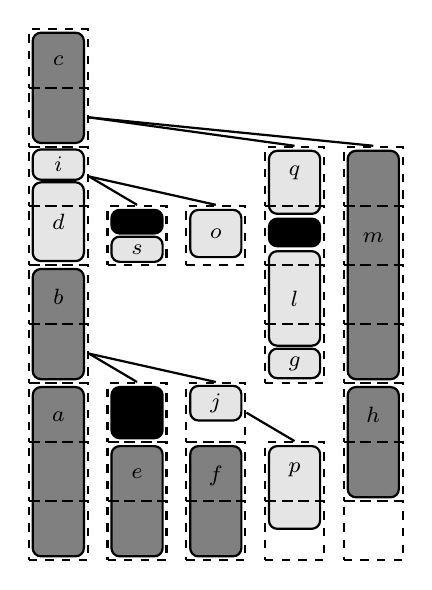
\begin{tikzpicture}[ every path/.style={thick}]
        \footnotesize
    \node[draw, 
        rounded corners=3pt, 
        minimum width=0.65cm, 
        minimum height=1.4cm, 
        align=center, fill=gray
        ] (A) at (0,-0.375) {\raisebox{0.7cm}{$c$}};

    \node[draw, 
        rounded corners=3pt, 
        minimum width=0.65cm, 
        minimum height=0.3cm, 
        align=center, fill=gray!20
        ] (A) at (0,-1.35) {$i$};
    
    \node[draw, 
        rounded corners=3pt, 
        minimum width=0.65cm, 
        minimum height=1.0cm, 
        align=center, fill=gray!20
        ] (A) at (0,-2.075) {$d$};

    \node[draw, 
        rounded corners=3pt, 
        minimum width=0.65cm, 
        minimum height=1.4cm, 
        align=center, fill=gray
        ] (A) at (0,-3.375) {\raisebox{0.7cm}{$b$}};

    \node[draw, 
        rounded corners=3pt, 
        minimum width=0.65cm, 
        minimum height=2.15cm, 
        align=center, fill=gray
        ] (A) at (0,-5.25) {\raisebox{1.4cm}{$a$}};

    \node[circle,  draw, dashed, rectangle, minimum size=0.75cm, inner sep=0pt] (11) at (0,0) {};

    \node[circle, draw, dashed, rectangle, minimum size=0.75cm, inner sep=0pt] (12) at (0,-0.75) {};

    \node[circle, draw, dashed, rectangle, minimum size=0.75cm, inner sep=0pt] (13) at (0,-1.5) {};

    \node[circle, draw, dashed, rectangle, minimum size=0.75cm, inner sep=0pt] (14) at (0,-2.25) {};

    \node[circle, draw, dashed, rectangle, minimum size=0.75cm, inner sep=0pt] (15) at (0,-3) {};

    \node[circle, draw, dashed, rectangle, minimum size=0.75cm, inner sep=0pt] (16) at (0,-3.75) {};

    \node[circle, draw, dashed, rectangle, minimum size=0.75cm, inner sep=0pt] (17) at (0,-4.5) {};

    \node[circle, draw, dashed, rectangle, minimum size=0.75cm, inner sep=0pt] (18) at (0,-5.25) {};
    
    \node[circle, draw, dashed, rectangle, minimum size=0.75cm, inner sep=0pt] (19) at (0,-6) {};

    \node[draw, 
        rounded corners=3pt, 
        minimum width=0.65cm, 
        minimum height=0.3cm, 
        align=center, fill=black
        ] (A) at (1,-2.075) {};
    
    \node[draw, 
        rounded corners=3pt, 
        minimum width=0.65cm, 
        minimum height=0.3cm, 
        align=center, fill=gray!20
        ] (A) at (1,-2.425) {$s$};
    
    \node[circle, draw, dashed, rectangle, minimum size=0.75cm, inner sep=0pt] (24) at (1,-2.25) {};

    \draw[] (13.east) to (24.north);

    \node[draw, 
        rounded corners=3pt, 
        minimum width=0.65cm, 
        minimum height=0.65cm, 
        align=center, fill=black
        ] (A) at (1,-4.5) {};

    \node[draw, 
        rounded corners=3pt, 
        minimum width=0.65cm, 
        minimum height=1.4cm, 
        align=center, fill=gray
        ] (A) at (1,-5.625) {\raisebox{0.7cm}{$e$}};

    \node[circle, draw, dashed, rectangle, minimum size=0.75cm, inner sep=0pt] (27) at (1,-4.5) {};

    \node[circle, draw, dashed, rectangle, minimum size=0.75cm, inner sep=0pt] (28) at (1,-5.25) {};
    
    \node[circle, draw, dashed, rectangle, minimum size=0.75cm, inner sep=0pt] (29) at (1,-6) {};

    \draw[] (16.east) to (27.north);

    \node[draw, 
        rounded corners=3pt, 
        minimum width=0.65cm, 
        minimum height=0.6cm, 
        align=center, fill=gray!20
        ] (A) at (2,-2.225) {$o$};
    
    \node[circle, draw, dashed, rectangle, minimum size=0.75cm, inner sep=0pt] (34) at (2,-2.25) {};

    \draw[] (13.east) to (34.north);

    \node[draw, 
        rounded corners=3pt, 
        minimum width=0.65cm, 
        minimum height=0.3cm, 
        align=center, fill=gray!20
        ] (A) at (2,-4.38) {$j$};
    
    \node[draw, 
        rounded corners=3pt, 
        minimum width=0.65cm, 
        minimum height=1.4cm, 
        align=center, fill=gray
        ] (A) at (2,-5.625) {\raisebox{0.7cm}{$f$}};

    \node[circle, draw, dashed, rectangle, minimum size=0.75cm, inner sep=0pt] (37) at (2,-4.5) {};

    \node[circle, draw, dashed, rectangle, minimum size=0.75cm, inner sep=0pt] (38) at (2,-5.25) {};
    
    \node[circle, draw, dashed, rectangle, minimum size=0.75cm, inner sep=0pt] (39) at (2,-6) {};

    \draw[] (16.east) to (37.north);

    
    \node[draw, 
        rounded corners=3pt, 
        minimum width=0.65cm, 
        minimum height=0.8cm, 
        align=center, fill=gray!20
        ] (A) at (3,-1.575) {\raisebox{0.3cm}{$q$}};

    \node[draw, 
        rounded corners=3pt, 
        minimum width=0.65cm, 
        minimum height=0.35cm, 
        align=center, fill=black
        ] (A) at (3,-2.212) {};


    \node[draw, 
        rounded corners=3pt, 
        minimum width=0.65cm, 
        minimum height=1.2cm, 
        align=center, fill=gray!20
        ] (A) at (3,-3.05) {$l$};

    \node[draw, 
        rounded corners=3pt, 
        minimum width=0.65cm, 
        minimum height=0.3cm, 
        align=center, fill=gray!20
        ] (A) at (3,-3.875) {$g$};

    \node[circle, draw, dashed, rectangle, minimum size=0.75cm, inner sep=0pt] (43) at (3,-1.5) {};

    \node[circle, draw, dashed, rectangle, minimum size=0.75cm, inner sep=0pt] (44) at (3,-2.25) {};
    
    \node[circle, draw, dashed, rectangle, minimum size=0.75cm, inner sep=0pt] (45) at (3,-3) {};

    \node[circle, draw, dashed, rectangle, minimum size=0.75cm, inner sep=0pt] (46) at (3,-3.75) {};

    \draw[] (12.east) to (43.north);

    \node[draw, 
        rounded corners=3pt, 
        minimum width=0.65cm, 
        minimum height=1.05cm, 
        align=center, fill=gray!20
        ] (A) at (3,-5.45) {\raisebox{0.5cm}{$p$}};

    \node[circle, draw, dashed, rectangle, minimum size=0.75cm, inner sep=0pt] (48) at (3,-5.25) {};
    
    \node[circle, draw, dashed, rectangle, minimum size=0.75cm, inner sep=0pt] (49) at (3,-6) {};

    \draw[] (37.east) to (48.north);

    \node[draw, 
        rounded corners=3pt, 
        minimum width=0.65cm, 
        minimum height=2.9cm, 
        align=center, fill=gray
        ] (A) at (4,-2.625) {\raisebox{0.7cm}{$m$}};

    \node[draw, 
        rounded corners=3pt, 
        minimum width=0.65cm, 
        minimum height=1.4cm, 
        align=center, fill=gray
        ] (A) at (4,-4.875) {\raisebox{0.7cm}{$h$}};

    \node[circle, draw, dashed, rectangle, minimum size=0.75cm, inner sep=0pt] (53) at (4,-1.5) {};

    \node[circle, draw, dashed, rectangle, minimum size=0.75cm, inner sep=0pt] (54) at (4,-2.25) {};

    \node[circle, draw, dashed, rectangle, minimum size=0.75cm, inner sep=0pt] (55) at (4,-3) {};

    \node[circle, draw, dashed, rectangle, minimum size=0.75cm, inner sep=0pt] (56) at (4,-3.75) {};

    \node[circle, draw, dashed, rectangle, minimum size=0.75cm, inner sep=0pt] (57) at (4,-4.5) {};

    \node[circle, draw, dashed, rectangle, minimum size=0.75cm, inner sep=0pt] (58) at (4,-5.25) {};
    
    \node[circle, draw, dashed, rectangle, minimum size=0.75cm, inner sep=0pt] (59) at (4,-6) {};

    \draw[] (12.east) to (53.north);
    
    \end{tikzpicture}
    \caption[Example boxed decision tree $D$]{}\label{box_dt}
\end{minipage}

\caption[Structure of a boxed decision tree]{Structure of a boxed decision tree. Figure \ref{box_dt_input} shows example input tree $T$, black vertices are heavy and white vertices are white. Figure \ref{box_dt} shows example boxed decision tree $D$ for $T$, dark gray queries are heavy, light gray queries are light, and black spaces represent additional load of boxes.}\label{box_dt_figure}
\end{figure}

To devise our dynamic programming procedure, we will need the following generalization of an hierarchical decision trees. A \textit{boxed decision tree} $D=\br{V\br{D}, E\br{D}, u, l}$ for the tree $T$ is a tuple, in which $V\br{D}$ are the nodes of the decision trees, which we will call \textit{boxes}, $E\br{D}$ are edges of the decision tree, $u:V\br{T}\times V\br{D}\to \brc{0, 1/pn,2/pn,\dots,k}$ is the \textit{usage} function and $l:V\br{D}\to\brc{0, 1/pn,2/pn,\dots,k}$ is the \textit{load} function. Based on $u$, for every $b\in V\br{D}$ we will also define the \textit{query assignment} as following: $Q\br{b}=\brc{v\in V\br{T}|u\br{v,b}>0}$, these are the vertices of $T$, such that queries to them overlap with the box $b$.

The boxed decision tree is defined analogously as ordinary decision tree, however, to each query in $b\in V\br{D}$ instead of one vertex of $V\br{T}$, we assign an arbitrary subset of $V\br{T}$, via the query assignment function $Q$. Let $b\in V\br{D}$, and let $T'$ be a candidate subtree of $T$ right before any vertex in $Q\br{b}$ was queried. A box $p$ is a left child of $b$, if either $b$ corresponds to a subtree $T''\in T-Q\br{b}$ such that $r\br{T'}\in V\br{T''}$ or $Q\br{b}\cup Q\br{p}\neq \emptyset$. If otherwise, then $p$ is a right child of $b$.

We demand that for every $v\in V\br{T}$, all boxes $b\in V\br{D}$, such that $v\in Q\br{b}$ form a connected path in $D$, in which every child is a left child, for any intererior box $b$ of this path, $l\br{b}=0$ and $u\br{v,b}=k$. We will also require that: for every $q\in V\br{D}$, $l\br{b}+\sum_{v\in V\br{T}}u\br{v,b}\leq k$ and for every $v\in V\br{T}$ either $\sum_{b\in V\br{D}}\br{v,b}=0$, in which case such query is called \textit{unassigned} or $\sum_{b\in V\br{D}}\br{v,b}=c\br{v}$ and the query is called \textit{assigned}. Since we want the boxed decision tree to also be aligned, we will demand that if for any vertex $v\in V\br{T}$, $c\br{v}>pk$, then for every $b\in V\br{D}$, either $u\br{v,b}=0$ or $u\br{v,b}=k$. 

We now define how to search in $T$ using a boxed decision tree $D$. Firstly, the query process stops for time $l\br{u}$. If $Q\br{r\br{D}}\cup V\br{T} = \emptyset$, then we recurse on the appropriate child of $r\br{T}$ (which corresponds to our current candidate subtree). Otherwise, we pick the least costly vertex $v$ in $Q\br{r\br{D}}$, we remove $v$ from $Q\br{q}$ for any $q\in V\br{D}$ and we recurse on the last box which contained a query to $v$ (note that this can also be $r\br{v}$). This is done in order to ensure that the start of the query $t_v$ of each vertex $v$ happens in the box containing it. The aligned cost of seaching using a boxed decision tree is defined analogously as the aligned cost of searching using ordinary decision tree. Note that any boxed decision tree, can also be transformed to an equivalent aligned decision tree with the same aligned cost of searching. Conversely, any aligned decision tree can be transformed into a boxed decision tree, by subdividing the queries into boxes according to the their starting points. Note that since we do not count the cost of light down responses, by sorting all queries starting in a given box according to their cost, we cannot increase the aligned cost.


\SetKwFunction{FDPTimelines}{DPTimelines}
\begin{figure}[htp]
    \begin{minipage}[t]{0.17\textwidth}
    \centering
    \begin{tikzpicture}[every node/.style={draw, very thick}, every path/.style={very thick}]
    
    \node[draw, 
        rounded corners=3pt, 
        minimum width=0.65cm, 
        minimum height=0.65cm, 
        align=center, fill=black, drop shadow
        ] (A) at (0,-0.75) {};

    \node[draw, 
        rounded corners=3pt, 
        minimum width=0.65cm, 
        minimum height=0.3cm, 
        align=center, fill=black, drop shadow
        ] (A) at (0,-1.325) {};

    \node[draw, 
        rounded corners=3pt, 
        minimum width=0.65cm, 
        minimum height=0.65cm, 
        align=center, fill=black, drop shadow
        ] (A) at (0,-3.75) {};
    
    \node[draw, 
        rounded corners=3pt, 
        minimum width=0.65cm, 
        minimum height=0.1cm, 
        align=center, fill=black, drop shadow
        ] (A) at (0,-4.3) {};
    
    
    \node[circle,  draw, dashed, rectangle, minimum size=0.75cm, inner sep=0pt] (11) at (0,0) {};

    \node[circle, draw, dashed, rectangle, minimum size=0.75cm, inner sep=0pt] (12) at (0,-0.75) {};

    \node[circle, draw, dashed, rectangle, minimum size=0.75cm, inner sep=0pt] (13) at (0,-1.5) {};

    \node[circle, draw, dashed, rectangle, minimum size=0.75cm, inner sep=0pt] (14) at (0,-2.25) {};

    \node[circle, draw, dashed, rectangle, minimum size=0.75cm, inner sep=0pt] (15) at (0,-3) {};

    \node[circle, draw, dashed, rectangle, minimum size=0.75cm, inner sep=0pt] (16) at (0,-3.75) {};

    \node[circle, draw, dashed, rectangle, minimum size=0.75cm, inner sep=0pt] (17) at (0,-4.5) {};

    \node[circle, draw, minimum size=0.15cm, inner sep=0pt, fill=white, thick
        ] (A) at (0.375,-0.375) {};

    \node[circle, draw, minimum size=0.15cm, inner sep=0pt, fill=black, thick
        ] (A) at (0.375,-1.125) {};

    \node[circle, draw, minimum size=0.15cm, inner sep=0pt, fill=white, thick
        ] (A) at (0.375,-1.875) {};
    
    \node[circle, draw, minimum size=0.15cm, inner sep=0pt, fill=white, thick
        ] (A) at (0.375,-2.625) {};

    \node[circle, draw, minimum size=0.15cm, inner sep=0pt, fill=white, thick
        ] (A) at (0.375,-3.375) {};

    \node[circle, draw, minimum size=0.15cm, inner sep=0pt, fill=white, thick
        ] (A) at (0.375,-4.125) {};

    \node[circle, draw, minimum size=0.15cm, inner sep=0pt, fill=white, thick
        ] (A) at (0.375,-4.875) {};

    \end{tikzpicture}
    \caption[Boxline $B$]{}\label{boxline}
\end{minipage}
\begin{minipage}[t]{0.27\textwidth}
    \centering
    
    \begin{tikzpicture}[every node/.style={draw, very thick}, every path/.style={very thick}]
    
    \node[draw, 
        rounded corners=3pt, 
        minimum width=0.65cm, 
        minimum height=0.65cm, 
        align=center, fill=black, drop shadow
        ] (A) at (0,-0.75) {};

    \node[draw, 
        rounded corners=3pt, 
        minimum width=0.65cm, 
        minimum height=0.65cm, 
        align=center, fill=black, drop shadow
        ] (A) at (0,-1.5) {};

    \node[draw, 
        rounded corners=3pt, 
        minimum width=0.65cm, 
        minimum height=0.1cm, 
        align=center, fill=black, drop shadow
        ] (A) at (0,-2.05) {};

    \node[draw, 
        rounded corners=3pt, 
        minimum width=0.65cm, 
        minimum height=0.45cm, 
        align=center, fill=black, drop shadow
        ] (A) at (0,-2.9) {};

    \node[draw, 
        rounded corners=3pt, 
        minimum width=0.65cm, 
        minimum height=0.65cm, 
        align=center, fill=black, drop shadow
        ] (A) at (0,-3.75) {};
    
    \node[draw, 
        rounded corners=3pt, 
        minimum width=0.65cm, 
        minimum height=0.45cm, 
        align=center, fill=black, drop shadow
        ] (A) at (0,-4.4) {};
    
    
    \node[circle,  draw, dashed, rectangle, minimum size=0.75cm, inner sep=0pt] (11) at (0,0) {};

    \node[circle, draw, dashed, rectangle, minimum size=0.75cm, inner sep=0pt] (12) at (0,-0.75) {};

    \node[circle, draw, dashed, rectangle, minimum size=0.75cm, inner sep=0pt] (13) at (0,-1.5) {};

    \node[circle, draw, dashed, rectangle, minimum size=0.75cm, inner sep=0pt] (14) at (0,-2.25) {};

    \node[circle, draw, dashed, rectangle, minimum size=0.75cm, inner sep=0pt] (15) at (0,-3) {};

    \node[circle, draw, dashed, rectangle, minimum size=0.75cm, inner sep=0pt] (16) at (0,-3.75) {};

    \node[circle, draw, dashed, rectangle, minimum size=0.75cm, inner sep=0pt] (17) at (0,-4.5) {};

    \node[circle, draw, minimum size=0.15cm, inner sep=0pt, fill=white, thick
        ] (A) at (0.375,-0.375) {};

    \node[circle, draw, minimum size=0.15cm, inner sep=0pt, fill=black, thick
        ] (A) at (0.375,-1.125) {};

    \node[circle, draw, minimum size=0.15cm, inner sep=0pt, fill=black, thick
        ] (A) at (0.375,-1.875) {};
    
    \node[circle, draw, minimum size=0.15cm, inner sep=0pt, fill=white, thick
        ] (A) at (0.375,-2.625) {};

    \node[circle, draw, minimum size=0.15cm, inner sep=0pt, fill=black, thick
        ] (A) at (0.375,-3.375) {};

    \node[circle, draw, minimum size=0.15cm, inner sep=0pt, fill=white, thick
        ] (A) at (0.375,-4.125) {};

    \node[circle, draw, minimum size=0.15cm, inner sep=0pt, fill=black, thick
        ] (A) at (0.375,-4.875) {};




    \node[draw, 
        rounded corners=3pt, 
        minimum width=0.65cm, 
        minimum height=0.65cm, 
        align=center, fill=black, drop shadow
        ] (A) at (2,0) {};

    \node[draw, 
        rounded corners=3pt, 
        minimum width=0.65cm, 
        minimum height=0.65cm, 
        align=center, fill=black, drop shadow
        ] (A) at (2,-0.75) {};

    \node[draw, 
        rounded corners=3pt, 
        minimum width=0.65cm, 
        minimum height=0.3cm, 
        align=center, fill=black, drop shadow
        ] (A) at (2,-1.325) {};

    \node[draw, 
        rounded corners=3pt, 
        minimum width=0.65cm, 
        minimum height=0.45cm, 
        align=center, fill=black, drop shadow
        ] (A) at (2,-2.15) {};

    \node[draw, 
        rounded corners=3pt, 
        minimum width=0.65cm, 
        minimum height=0.1cm, 
        align=center, fill=black, drop shadow
        ] (A) at (2,-2.8) {};

    \node[draw, 
        rounded corners=3pt, 
        minimum width=0.65cm, 
        minimum height=0.65cm, 
        align=center, fill=black, drop shadow
        ] (A) at (2,-3.75) {};
        
    
    \node[draw, 
        rounded corners=3pt, 
        minimum width=0.65cm, 
        minimum height=0.45cm, 
        align=center, fill=black, drop shadow
        ] (A) at (2,-4.4) {};
    
    
    \node[circle,  draw, dashed, rectangle, minimum size=0.75cm, inner sep=0pt] (11) at (2,0) {};

    \node[circle, draw, dashed, rectangle, minimum size=0.75cm, inner sep=0pt] (12) at (2,-0.75) {};

    \node[circle, draw, dashed, rectangle, minimum size=0.75cm, inner sep=0pt] (13) at (2,-1.5) {};

    \node[circle, draw, dashed, rectangle, minimum size=0.75cm, inner sep=0pt] (14) at (2,-2.25) {};

    \node[circle, draw, dashed, rectangle, minimum size=0.75cm, inner sep=0pt] (15) at (2,-3) {};

    \node[circle, draw, dashed, rectangle, minimum size=0.75cm, inner sep=0pt] (16) at (2,-3.75) {};

    \node[circle, draw, dashed, rectangle, minimum size=0.75cm, inner sep=0pt] (17) at (2,-4.5) {};

    \node[circle, draw, minimum size=0.15cm, inner sep=0pt, fill=black, thick
        ] (A) at (2.375,-0.375) {};

    \node[circle, draw, minimum size=0.15cm, inner sep=0pt, fill=black, thick
        ] (A) at (2.375,-1.125) {};

    \node[circle, draw, minimum size=0.15cm, inner sep=0pt, fill=white, thick
        ] (A) at (2.375,-1.875) {};
    
    \node[circle, draw, minimum size=0.15cm, inner sep=0pt, fill=black, thick
        ] (A) at (2.375,-2.625) {};

    \node[circle, draw, minimum size=0.15cm, inner sep=0pt, fill=white, thick
        ] (A) at (2.375,-3.375) {};

    \node[circle, draw, minimum size=0.15cm, inner sep=0pt, fill=black, thick
        ] (A) at (2.375,-4.125) {};

    \node[circle, draw, minimum size=0.15cm, inner sep=0pt, fill=white, thick
        ] (A) at (2.375,-4.875) {};

    \end{tikzpicture}
    \caption[Bipartition of $B$]{}\label{bipartition_boxline}
\end{minipage}
\begin{minipage}[t]{0.37\textwidth}
    \centering
    \begin{tikzpicture}[every path/.style={very thick}]
    \footnotesize

    \node[draw, 
        rounded corners=3pt, 
        minimum width=0.65cm, 
        minimum height=0.1cm, 
        align=center, fill=gray!20, drop shadow
        ] (A) at (-2.5,0.225) {};

    \node[draw, 
        rounded corners=3pt, 
        minimum width=0.65cm, 
        minimum height=0.25cm, 
        align=center, fill=gray!20, drop shadow
        ] (A) at (-2.5,-0.05) {};

    \node[draw, 
        rounded corners=3pt, 
        minimum width=0.65cm, 
        minimum height=0.65cm, 
        align=center, fill=black, drop shadow
        ] (A) at (-2.5,-0.75) {};

    \node[draw, 
        rounded corners=3pt, 
        minimum width=0.65cm, 
        minimum height=0.65cm, 
        align=center, fill=black, drop shadow
        ] (A) at (-2.5,-1.5) {};

    \node[draw, 
        rounded corners=3pt, 
        minimum width=0.65cm, 
        minimum height=0.1cm, 
        align=center, fill=black, drop shadow
        ] (A) at (-2.5,-2.025) {};

    \node[draw, 
        rounded corners=3pt, 
        minimum width=0.65cm, 
        minimum height=0.63cm, 
        align=center, fill=gray!20, drop shadow
        ] (A) at (-2.5,-2.5) {\raisebox{0.15cm}{$v$}};

    \node[draw, 
        rounded corners=3pt, 
        minimum width=0.65cm, 
        minimum height=0.45cm, 
        align=center, fill=black, drop shadow
        ] (A) at (-2.5,-3.1) {};


    \node[draw, 
        rounded corners=3pt, 
        minimum width=0.65cm, 
        minimum height=0.65cm, 
        align=center, fill=black, drop shadow
        ] (A) at (-2.5,-3.75) {};
    
    \node[draw, 
        rounded corners=3pt, 
        minimum width=0.65cm, 
        minimum height=0.45cm, 
        align=center, fill=black, drop shadow
        ] (A) at (-2.5,-4.4) {};
    
    
    \node[circle,  draw, dashed, rectangle, minimum size=0.75cm, inner sep=0pt] (11) at (-2.5,0) {};

    \node[circle, draw, dashed, rectangle, minimum size=0.75cm, inner sep=0pt] (12) at (-2.5,-0.75) {};

    \node[circle, draw, dashed, rectangle, minimum size=0.75cm, inner sep=0pt] (13) at (-2.5,-1.5) {};

    \node[circle, draw, dashed, rectangle, minimum size=0.75cm, inner sep=0pt] (14) at (-2.5,-2.25) {};

    \node[circle, draw, dashed, rectangle, minimum size=0.75cm, inner sep=0pt] (15) at (-2.5,-3) {};

    \node[circle, draw, dashed, rectangle, minimum size=0.75cm, inner sep=0pt] (16) at (-2.5,-3.75) {};

    \node[circle, draw, dashed, rectangle, minimum size=0.75cm, inner sep=0pt] (17) at (-2.5,-4.5) {};

    \draw[very thick, fill=gray!20, drop shadow] (-1.5,-1) -- (-1.8,-1.6) -- (-1.2,-1.6) -- cycle;

    \draw[very thick, fill=gray!20, drop shadow] (-0.5,-0.9) -- (-0.1,-1.7) -- (-0.9,-1.7) -- cycle;


    \node at (0.15, -1.25) {$\dots$}; 

    \draw[very thick, fill=gray!20, drop shadow] (0.8,-0.8) -- (0.3,-1.8) -- (1.3,-1.8) -- cycle;

    \draw[very thick] (11.east) -- (-1.5,-1);
    \draw[very thick] (11.east) -- (-0.5,-0.9);
    \draw[very thick] (11.east) -- (0.8,-0.8);

    \draw[very thick, fill=gray!20, drop shadow] (-1.2,-3.3) -- (-1.8,-4.5) -- (-0.6,-4.5) -- cycle;

    \draw[very thick, fill=gray!20, drop shadow] (0.4,-3.2) -- (-0.3,-4.6) -- (1.1,-4.6) -- cycle;

    \draw[very thick] (15.east) -- (-1.2,-3.3);
    
    \draw[very thick] (15.east) -- (0.4,-3.2);

    \end{tikzpicture}
    \caption[Decision tree $D_1$]{}\label{D1_boxline}
\end{minipage}
\begin{minipage}[t]{0.15\textwidth}
    \centering
    \begin{tikzpicture}[every path/.style={very thick}]
    
    


    \node[draw, 
        rounded corners=3pt, 
        minimum width=0.65cm, 
        minimum height=0.65cm, 
        align=center, fill=black, drop shadow
        ] (A) at (2,0) {};

    \node[draw, 
        rounded corners=3pt, 
        minimum width=0.65cm, 
        minimum height=0.65cm, 
        align=center, fill=black, drop shadow
        ] (A) at (2,-0.75) {};

    \node[draw, 
        rounded corners=3pt, 
        minimum width=0.65cm, 
        minimum height=0.3cm, 
        align=center, fill=black, drop shadow
        ] (A) at (2,-1.325) {};

    \node[draw, 
        rounded corners=3pt, 
        minimum width=0.65cm, 
        minimum height=0.45cm, 
        align=center, fill=black, drop shadow
        ] (A) at (2,-2.15) {};

    \node[draw, 
        rounded corners=3pt, 
        minimum width=0.65cm, 
        minimum height=0.1cm, 
        align=center, fill=black, drop shadow
        ] (A) at (2,-2.8) {};

    
    
    \node[circle,  draw, dashed, rectangle, minimum size=0.75cm, inner sep=0pt] (11) at (2,0) {};

    \node[circle, draw, dashed, rectangle, minimum size=0.75cm, inner sep=0pt] (12) at (2,-0.75) {};

    \node[circle, draw, dashed, rectangle, minimum size=0.75cm, inner sep=0pt] (13) at (2,-1.5) {};

    \node[circle, draw, dashed, rectangle, minimum size=0.75cm, inner sep=0pt] (14) at (2,-2.25) {};

    \node[circle, draw, dashed, rectangle, minimum size=0.75cm, inner sep=0pt] (15) at (2,-3) {};

    \node[circle, draw, dashed, rectangle, minimum size=0.75cm, inner sep=0pt] (16) at (2,-3.75) {};

    \node[circle, draw, dashed, rectangle, minimum size=0.75cm, inner sep=0pt] (17) at (2,-4.5) {};

    \node[circle, draw, minimum size=0.15cm, inner sep=0pt, fill=black, thick
        ] (A) at (2.375,-0.375) {};

    \node[circle, draw, minimum size=0.15cm, inner sep=0pt, fill=black, thick
        ] (A) at (2.375,-1.125) {};

    \node[circle, draw, minimum size=0.15cm, inner sep=0pt, fill=white, thick
        ] (A) at (2.375,-1.875) {};
    
    \node[circle, draw, minimum size=0.15cm, inner sep=0pt, fill=black, thick
        ] (A) at (2.375,-2.625) {};

    \node[circle, draw, minimum size=0.15cm, inner sep=0pt, fill=white, thick
        ] (A) at (2.375,-3.375) {};

    \node[circle, draw, minimum size=0.15cm, inner sep=0pt, fill=white, thick
        ] (A) at (2.375,-4.125) {};

    \node[circle, draw, minimum size=0.15cm, inner sep=0pt, fill=white, thick
        ] (A) at (2.375,-4.875) {};


    \end{tikzpicture}
    \caption[Boxline $B_2$]{}\label{B2_boxline}
\end{minipage}

\begin{minipage}[t]{0.3\textwidth}
    \centering
    \begin{tikzpicture}[every path/.style={very thick}]
    
    
    \node[draw, 
        rounded corners=3pt, 
        minimum width=0.65cm, 
        minimum height=0.65cm, 
        align=center, fill=black, drop shadow
        ] (A) at (0,0) {};

    \node[draw, 
        rounded corners=3pt, 
        minimum width=0.65cm, 
        minimum height=0.65cm, 
        align=center, fill=black, drop shadow
        ] (A) at (0,-0.75) {};

    \node[draw, 
        rounded corners=3pt, 
        minimum width=0.65cm, 
        minimum height=0.3cm, 
        align=center, fill=black, drop shadow
        ] (A) at (0,-1.325) {};

    \node[draw, 
        rounded corners=3pt, 
        minimum width=0.65cm, 
        minimum height=0.3cm, 
        align=center, fill=gray!20, drop shadow
        ] (A) at (0,-1.68) {};

    \node[draw, 
        rounded corners=3pt, 
        minimum width=0.65cm, 
        minimum height=0.45cm, 
        align=center, fill=black, drop shadow
        ] (A) at (0,-2.15) {};

    \node[draw, 
        rounded corners=3pt, 
        minimum width=0.65cm, 
        minimum height=0.1cm, 
        align=center, fill=black, drop shadow
        ] (A) at (0,-2.8) {};

    \node[draw, 
        rounded corners=3pt, 
        minimum width=0.65cm, 
        minimum height=0.35cm, 
        align=center, fill=gray!20, drop shadow
        ] (A) at (0,-3.15) {};

    \node[draw, 
        rounded corners=3pt, 
        minimum width=0.65cm, 
        minimum height=0.65cm, 
        align=center, fill=gray!20, drop shadow
        ] (A) at (0,-3.75) {};

    
    
    \node[circle,  draw, dashed, rectangle, minimum size=0.75cm, inner sep=0pt] (11) at (0,0) {};

    \node[circle, draw, dashed, rectangle, minimum size=0.75cm, inner sep=0pt] (12) at (0,-0.75) {};

    \node[circle, draw, dashed, rectangle, minimum size=0.75cm, inner sep=0pt] (13) at (0,-1.5) {};

    \node[circle, draw, dashed, rectangle, minimum size=0.75cm, inner sep=0pt] (14) at (0,-2.25) {};

    \node[circle, draw, dashed, rectangle, minimum size=0.75cm, inner sep=0pt] (15) at (0,-3) {};

    \node[circle, draw, dashed, rectangle, minimum size=0.75cm, inner sep=0pt] (16) at (0,-3.75) {};

    \node[circle, draw, dashed, rectangle, minimum size=0.75cm, inner sep=0pt] (17) at (0,-4.5) {};
    
    \draw[very thick, fill=white, drop shadow] (1.5,-2.5) -- (1.9,-3.3) -- (1.1,-3.3) -- cycle;

    \draw[very thick, fill=white, drop shadow] (2.7,-2.4) -- (2.2,-3.4) -- (3.2,-3.4) -- cycle;

    \draw[very thick] (13.east) -- (1.5,-2.5);
    
    \draw[very thick] (13.east) -- (2.7,-2.4);

    \draw[very thick, fill=white, drop shadow] (2,-4) -- (1.5,-5) -- (2.5,-5) -- cycle;

    \draw[very thick] (15.east) -- (2,-4);

    \draw[very thick, fill=white, drop shadow] (1,-4.3) -- (1.3,-4.9) -- (0.7,-4.9) -- cycle;

    \draw[very thick] (16.east) -- (1,-4.3);

    \end{tikzpicture}
    \caption[Decision tree $D_2$]{}\label{D2_boxline}
\end{minipage}
\begin{minipage}[t]{0.3\textwidth}
    \centering
    \begin{tikzpicture}[every path/.style={very thick}]
    
    
    \node[draw, 
        rounded corners=3pt, 
        minimum width=0.65cm, 
        minimum height=0.65cm, 
        align=center, fill=black, drop shadow
        ] (A) at (0,0) {};

    \node[draw, 
        rounded corners=3pt, 
        minimum width=0.65cm, 
        minimum height=0.65cm, 
        align=center, fill=black, drop shadow
        ] (A) at (0,-0.75) {};

    \node[draw, 
        rounded corners=3pt, 
        minimum width=0.65cm, 
        minimum height=0.3cm, 
        align=center, fill=black, drop shadow
        ] (A) at (0,-1.325) {};

    \node[draw, 
        rounded corners=3pt, 
        minimum width=0.65cm, 
        minimum height=0.3cm, 
        align=center, fill=gray!20, drop shadow
        ] (A) at (0,-1.68) {};

    \node[draw, 
        rounded corners=3pt, 
        minimum width=0.65cm, 
        minimum height=0.45cm, 
        align=center, fill=black, drop shadow
        ] (A) at (0,-2.15) {};

    \node[draw, 
        rounded corners=3pt, 
        minimum width=0.65cm, 
        minimum height=0.1cm, 
        align=center, fill=black, drop shadow
        ] (A) at (0,-2.8) {};

    \node[draw, 
        rounded corners=3pt, 
        minimum width=0.65cm, 
        minimum height=0.35cm, 
        align=center, fill=gray!20, drop shadow
        ] (A) at (1,-3.575) {};

    \node[draw, 
        rounded corners=3pt, 
        minimum width=0.65cm, 
        minimum height=0.65cm, 
        align=center, fill=gray!20, drop shadow
        ] (A) at (1,-4.5) {};

    
    
    \node[circle,  draw, dashed, rectangle, minimum size=0.75cm, inner sep=0pt] (11) at (0,0) {};

    \node[circle, draw, dashed, rectangle, minimum size=0.75cm, inner sep=0pt] (12) at (0,-0.75) {};

    \node[circle, draw, dashed, rectangle, minimum size=0.75cm, inner sep=0pt] (13) at (0,-1.5) {};

    \node[circle, draw, dashed, rectangle, minimum size=0.75cm, inner sep=0pt] (14) at (0,-2.25) {};

    \node[circle, draw, dashed, rectangle, minimum size=0.75cm, inner sep=0pt] (15) at (0,-3) {};

    
    \node[circle, draw, dashed, rectangle, minimum size=0.75cm, inner sep=0pt] (26) at (1,-3.75) {};

    \node[circle, draw, dashed, rectangle, minimum size=0.75cm, inner sep=0pt] (27) at (1,-4.5) {};

    \node[circle, draw, dashed, rectangle, minimum size=0.75cm, inner sep=0pt] (28) at (1,-5.25) {};

    \draw[very thick] (15.east) -- (26.north);
    
    \draw[very thick, fill=white, drop shadow] (1,-2) -- (1.4,-2.8) -- (0.6,-2.8) -- cycle;

    \draw[very thick, fill=white, drop shadow] (2.2,-1.9) -- (1.7,-2.9) -- (2.7,-2.9) -- cycle;

    \draw[very thick] (13.east) -- (1,-2);
    
    \draw[very thick] (13.east) -- (2.2,-1.9);

    \draw[very thick, fill=white, drop shadow] (3,-4.5) -- (2.5,-5.5) -- (3.5,-5.5) -- cycle;

    \draw[very thick] (26.east) -- (3,-4.5);

    \draw[very thick, fill=white, drop shadow] (2,-4.8) -- (2.3,-5.4) -- (1.7,-5.4) -- cycle;

    \draw[very thick] (27.east) -- (2,-4.8);


    \end{tikzpicture}
    \caption[Rehanging step]{}\label{rehang_boxline}
\end{minipage}
\begin{minipage}[t]{0.4\textwidth}
    \centering
    \begin{tikzpicture}[every path/.style={very thick}]
    \footnotesize
    \node[draw, 
        rounded corners=3pt, 
        minimum width=0.65cm, 
        minimum height=0.1cm, 
        align=center, fill=gray!20, drop shadow
        ] (A) at (-2.5,0.225) {};

    \node[draw, 
        rounded corners=3pt, 
        minimum width=0.65cm, 
        minimum height=0.25cm, 
        align=center, fill=gray!20, drop shadow
        ] (A) at (-2.5,-0.05) {};

    \node[draw, 
        rounded corners=3pt, 
        minimum width=0.65cm, 
        minimum height=0.65cm, 
        align=center, fill=black, drop shadow
        ] (A) at (-2.5,-0.75) {};

    \node[draw, 
        rounded corners=3pt, 
        minimum width=0.65cm, 
        minimum height=0.3cm, 
        align=center, fill=black, drop shadow
        ] (A) at (-2.5,-1.325) {};

    \node[draw, 
        rounded corners=3pt, 
        minimum width=0.65cm, 
        minimum height=0.3cm, 
        align=center, fill=gray!20, drop shadow
        ] (A) at (-2.5,-1.68) {};

    \node[draw, 
        rounded corners=3pt, 
        minimum width=0.65cm, 
        minimum height=0.63cm, 
        align=center, fill=gray!20, drop shadow
        ] (A) at (-2.5,-2.5) {\raisebox{0.15cm}{$v$}};

    \node[draw, 
        rounded corners=3pt, 
        minimum width=0.65cm, 
        minimum height=0.65cm, 
        align=center, fill=black, drop shadow
        ] (A) at (-2.5,-3.75) {};
    
    \node[draw, 
        rounded corners=3pt, 
        minimum width=0.65cm, 
        minimum height=0.1cm, 
        align=center, fill=black, drop shadow
        ] (A) at (-2.5,-4.3) {};

    
    \node[draw, 
        rounded corners=3pt, 
        minimum width=0.65cm, 
        minimum height=0.35cm, 
        align=center, fill=gray!20, drop shadow
        ] (A) at (-1.5,-3.575) {};

    \node[draw, 
        rounded corners=3pt, 
        minimum width=0.65cm, 
        minimum height=0.65cm, 
        align=center, fill=gray!20, drop shadow
        ] (A) at (-1.5,-4.5) {};
    
    
    \node[circle,  draw, dashed, rectangle, minimum size=0.75cm, inner sep=0pt] (11) at (-2.5,0) {};

    \node[circle, draw, dashed, rectangle, minimum size=0.75cm, inner sep=0pt] (12) at (-2.5,-0.75) {};

    \node[circle, draw, dashed, rectangle, minimum size=0.75cm, inner sep=0pt] (13) at (-2.5,-1.5) {};

    \node[circle, draw, dashed, rectangle, minimum size=0.75cm, inner sep=0pt] (14) at (-2.5,-2.25) {};

    \node[circle, draw, dashed, rectangle, minimum size=0.75cm, inner sep=0pt] (15) at (-2.5,-3) {};

    \node[circle, draw, dashed, rectangle, minimum size=0.75cm, inner sep=0pt] (16) at (-2.5,-3.75) {};

    \node[circle, draw, dashed, rectangle, minimum size=0.75cm, inner sep=0pt] (17) at (-2.5,-4.5) {};
;

    \node[circle, draw, dashed, rectangle, minimum size=0.75cm, inner sep=0pt] (26) at (-1.5,-3.75) {};

    \node[circle, draw, dashed, rectangle, minimum size=0.75cm, inner sep=0pt] (27) at (-1.5,-4.5) {};

    \node[circle, draw, dashed, rectangle, minimum size=0.75cm, inner sep=0pt] (28) at (-1.5,-5.25) {};

    \draw[very thick] (15.east) -- (26.north);


    \draw[very thick, fill=gray!20, drop shadow] (-1.5,-0.5) -- (-1.8,-1.1) -- (-1.2,-1.1) -- cycle;

    \draw[very thick, fill=gray!20, drop shadow] (-0.5,-0.4) -- (-0.1,-1.2) -- (-0.9,-1.2) -- cycle;


    \node at (0.15, -0.75) {$\dots$}; 

    \draw[very thick, fill=gray!20, drop shadow] (0.8,-0.3) -- (0.3,-1.3) -- (1.3,-1.3) -- cycle;

    \draw[very thick] (11.east) -- (-1.5,-0.5);
    \draw[very thick] (11.east) -- (-0.5,-0.4);
    \draw[very thick] (11.east) -- (0.8,-0.3);

    \draw[very thick, fill=gray!20, drop shadow] (0.3,-3.3) -- (-0.2,-4.3) -- (0.8,-4.3) -- cycle;

    \draw[very thick, fill=gray!20, drop shadow] (1.7,-3.2) -- (1.1,-4.4) -- (2.3,-4.4) -- cycle;

    \draw[very thick] (15.east) -- (0.3,-3.3);
    
    \draw[very thick] (15.east) -- (1.7,-3.2);

    \draw[very thick, fill=white, drop shadow] (-1,-2) -- (-0.6,-2.8) -- (-1.4,-2.8) -- cycle;

    \draw[very thick, fill=white, drop shadow] (0.2,-1.9) -- (-0.3,-2.9) -- (0.7,-2.9) -- cycle;

    \draw[very thick] (13.east) -- (-1,-2);
    
    \draw[very thick] (13.east) -- (0.2,-1.9);

    \draw[very thick, fill=white, drop shadow] (0.2,-4.9) -- (-0.2,-5.7) -- (0.6,-5.7) -- cycle;

    \draw[very thick] (26.east) -- (0.2,-4.9);

    \draw[very thick, fill=white, drop shadow] (-0.7,-5) -- (-0.4,-5.6) -- (-1,-5.6) -- cycle;

    \draw[very thick] (27.east) -- (-0.7,-5);

    \end{tikzpicture}
    \caption[Resulting decision tree $D$]{}\label{D_boxline}
\end{minipage}
\caption[Basic steps of \texttt{DPTimelines} procedure]{Basic steps of the case when $i>1$. The black regions represent the load of a box. Fig. \ref{boxline}: example boxline $B$. Fig. \ref{bipartition_boxline}: boxlines $B_1$ and $B_2$ induced by bipartitioning $B$. Fig \ref{D1_boxline}: decision tree $D_1$ box-compatible with timeline $B_1$. Fig \ref{P2}: timeline $B_2$ after deleting loads of nodes with indices below $k$. Fig \ref{D2_boxline}: a decision tree $D_2$ compatible with $B_2$. Fig \ref{rehang_boxline}: $D_2$ with left child of $q_k$ rehanged to right. Fig \ref{D_boxline}: $D_1$ and $D_2$ aligned by their left box-paths.}\label{dp_timelines_costs_figure}
\end{figure}

We define a \textit{boxline} $B\angl{\br{b_1, \tau_1},\br{b_2, \tau_2},\dots, \br{b_d, \tau_d}}$ to be a sequence of pairs, each consisting of box and additional boolean flag, such that for every box $b$ in $B$, $Q\br{b}=\emptyset$. We will build our decision trees around boxlines. Define the \textit{left box-path} $B_D=\angl{{q_1, f_1},\br{q_2, f_2},\dots, \br{q_h, f_h}}$ of $D$ as a sequence of pairs. Each such pair consisits of the overall loads of consecutive boxes obtained by traversing $D$ starting from root $r\br{D}$, and stepping to the left child until there is none (for each such box $b$ with index $j$, $q_j=l\br{b}+\sum_{v\in Q\br{b}}q\br{v, b}$), and boolean values denoting whether there exists a query trascending the current box unto the next one ($f_h$ is always false, however we include it for convenience). We will say that a decision tree $D$ with a left box-path $B_D$ is \textit{box-compatible} with a boxline $B$, such that $h\leq d$, if for every integer $1\leq j \leq h$, $l\br{q_j}\geq l\br{b_j}$ and if $\tau_j$ implies $f_j$. To build a decision $D$ tree using $B$, we simply create a boxed decision tree $D$ consisiting of path of vertices $\angl{q_1,\dots, q_h}$, such that $l\br{q_j}=l\br{b_j}$ and $Q\br{q_j}=\emptyset$.

We will also use the following operations: 
\begin{itemize}
    \item Puting a query to vertex $v$ at $s$-th slot of a box $b$:
    \begin{enumerate}
        \item $\sigma\br{v}\gets c\br{v}$: 
        \item \textbf{while} $\sigma\br{v}>0$: 
        \begin{enumerate}
            \item $u\br{v, b}\gets\min\brc{k-s/pn, \sigma\br{v}}$.
            \item $\sigma\br{v}\gets \sigma\br{v}-u\br{v, b}$. 
            \item $b\gets$ left child of $b$.
        \end{enumerate}
    \end{enumerate} If such operation violates the definition of $D$ or query to $v$ transcendents any box $b_j$, such that $\tau_j$ we mark $D$ as \textit{conflicted}.  
    \item Building a decision tree $D$ based on boxline $B$:
    \begin{enumerate}
        \item $D\gets\emptyset$.
        \item \textbf{for} $1\leq j\leq \spr{B}$:
        \begin{enumerate}
            \item Create box $q_j$ in $D$.
            \item $l\br{j}\gets b_j$.
            \item $Q\br{q_j}\gets\emptyset$.
            \item \textbf{if} $j>1$ \textbf{then}: hang $q_j$ as the left child of $q_{j-1}$.
        \end{enumerate}
        \item \textbf{return} $D$.
    \end{enumerate} 
    \item Rotating a decision tree $D$ around vertex $v\in V\br{D}$: 
    \begin{enumerate}
        \item $q_h\gets $ the box containing the end of query to $v$.
        \item Sort queries starting in $Q\br{q_h}$ according to $c'$.
        \item Create box $q$.
        \item Move queries from $Q\br{q_h}$ to $Q\br{q}$, so that all queries after $v$ are in $Q\br{q}$.
        \item Hang $q_h'$ as a right child of $q_h$.
        \item Rehang left child of $q_h$ as the left child of $q$. 
    \end{enumerate}
    
    \item Bipartitioning of $B$. A bipartition of a boxline $B$ consists of a pair of boxlines $\br{B_1,B_2}$ such that:
    \begin{itemize}
        \item $\spr{B}=\spr{B_1}=\spr{B_2}$.
        \item $l\br{b_{1,j}}+l\br{b_{2,j}} - k = l\br{b_j}$.
        \item $\br{\tau_{1,j}\land \tau_{2,j} \iff \tau_{j}}$.
        \item$\br{\tau_{1,j}\lor \tau_{2,j}}$.
    \end{itemize} 
    \item Aligning $D_1$ and $D_2$ by their left paths to create new decision tree $D$: 
    \begin{enumerate}
        \item $D\gets\emptyset$.
        \item \textbf{for} $1\leq j\leq \spr{B}$:
        \begin{enumerate}
            \item Create box $q_j$ in $D$.
            \item $l\br{j}\gets l\br{q_{1,j}}+ l\br{q_{2,j}}-k$.
            \item \textbf{for} $v\in V\br{T}$: $u\br{v, q_j}\gets \max\brc{u\br{v, q_{1,j}},u\br{v, q_{2,j}}}$.
            \item Hang all right children of $q_{1,j}$ and $q_{2,j}$ below $q_j$.
            \item \textbf{if} $j>1$ \textbf{then}: hang $q_j$ as the left child of $q_{j-1}$.
        \end{enumerate}
        \item \textbf{return} $D$.
    \end{enumerate}
\end{itemize}

We now introduce the subproblems which our dynamic programming solves. A problem $\OPT'\br{T_{v,i},B}$ consists of finding an optimal boxed decision tree for the tree $T_{v,i}$, which is box-compatible with $B$. If no $B$ is given, we assume that $B=\angl{\br{b_1,\tau_1},\dots, {b_d,\tau_d}}$, where for every $1\leq j\leq d$, $b_j=0$ and $\tau_j$ is false.
 The algorithm computes the solutions in a bottom-up, left-to-right manner. If at any point there is no way to create an extended decision tree with given parameters we simply declare such instance \textit{unfeasible}. We will now show how to compute $\OPT\br{T_{v,i}, B}$ efficiently. The Algorithm \ref{dp_timelines_costs} consists of 3 cases:
 

\SetKwFunction{FDPTimelines}{DPTimelines}
\begin{figure}[htp]
    \begin{minipage}[t]{0.17\textwidth}
    \centering
    \begin{tikzpicture}[every node/.style={draw, very thick}, every path/.style={very thick}]
    
    \node[draw, 
        rounded corners=3pt, 
        minimum width=0.65cm, 
        minimum height=0.65cm, 
        align=center, fill=black, drop shadow
        ] (A) at (0,-0.75) {};

    \node[draw, 
        rounded corners=3pt, 
        minimum width=0.65cm, 
        minimum height=0.3cm, 
        align=center, fill=black, drop shadow
        ] (A) at (0,-1.325) {};

    \node[draw, 
        rounded corners=3pt, 
        minimum width=0.65cm, 
        minimum height=0.65cm, 
        align=center, fill=black, drop shadow
        ] (A) at (0,-3.75) {};
    
    \node[draw, 
        rounded corners=3pt, 
        minimum width=0.65cm, 
        minimum height=0.1cm, 
        align=center, fill=black, drop shadow
        ] (A) at (0,-4.3) {};
    
    
    \node[circle,  draw, dashed, rectangle, minimum size=0.75cm, inner sep=0pt] (11) at (0,0) {};

    \node[circle, draw, dashed, rectangle, minimum size=0.75cm, inner sep=0pt] (12) at (0,-0.75) {};

    \node[circle, draw, dashed, rectangle, minimum size=0.75cm, inner sep=0pt] (13) at (0,-1.5) {};

    \node[circle, draw, dashed, rectangle, minimum size=0.75cm, inner sep=0pt] (14) at (0,-2.25) {};

    \node[circle, draw, dashed, rectangle, minimum size=0.75cm, inner sep=0pt] (15) at (0,-3) {};

    \node[circle, draw, dashed, rectangle, minimum size=0.75cm, inner sep=0pt] (16) at (0,-3.75) {};

    \node[circle, draw, dashed, rectangle, minimum size=0.75cm, inner sep=0pt] (17) at (0,-4.5) {};

    \node[circle, draw, minimum size=0.15cm, inner sep=0pt, fill=white, thick
        ] (A) at (0.375,-0.375) {};

    \node[circle, draw, minimum size=0.15cm, inner sep=0pt, fill=black, thick
        ] (A) at (0.375,-1.125) {};

    \node[circle, draw, minimum size=0.15cm, inner sep=0pt, fill=white, thick
        ] (A) at (0.375,-1.875) {};
    
    \node[circle, draw, minimum size=0.15cm, inner sep=0pt, fill=white, thick
        ] (A) at (0.375,-2.625) {};

    \node[circle, draw, minimum size=0.15cm, inner sep=0pt, fill=white, thick
        ] (A) at (0.375,-3.375) {};

    \node[circle, draw, minimum size=0.15cm, inner sep=0pt, fill=white, thick
        ] (A) at (0.375,-4.125) {};

    \node[circle, draw, minimum size=0.15cm, inner sep=0pt, fill=white, thick
        ] (A) at (0.375,-4.875) {};

    \end{tikzpicture}
    \caption[Boxline $B$]{}\label{boxline}
\end{minipage}
\begin{minipage}[t]{0.27\textwidth}
    \centering
    
    \begin{tikzpicture}[every node/.style={draw, very thick}, every path/.style={very thick}]
    
    \node[draw, 
        rounded corners=3pt, 
        minimum width=0.65cm, 
        minimum height=0.65cm, 
        align=center, fill=black, drop shadow
        ] (A) at (0,-0.75) {};

    \node[draw, 
        rounded corners=3pt, 
        minimum width=0.65cm, 
        minimum height=0.65cm, 
        align=center, fill=black, drop shadow
        ] (A) at (0,-1.5) {};

    \node[draw, 
        rounded corners=3pt, 
        minimum width=0.65cm, 
        minimum height=0.1cm, 
        align=center, fill=black, drop shadow
        ] (A) at (0,-2.05) {};

    \node[draw, 
        rounded corners=3pt, 
        minimum width=0.65cm, 
        minimum height=0.45cm, 
        align=center, fill=black, drop shadow
        ] (A) at (0,-2.9) {};

    \node[draw, 
        rounded corners=3pt, 
        minimum width=0.65cm, 
        minimum height=0.65cm, 
        align=center, fill=black, drop shadow
        ] (A) at (0,-3.75) {};
    
    \node[draw, 
        rounded corners=3pt, 
        minimum width=0.65cm, 
        minimum height=0.45cm, 
        align=center, fill=black, drop shadow
        ] (A) at (0,-4.4) {};
    
    
    \node[circle,  draw, dashed, rectangle, minimum size=0.75cm, inner sep=0pt] (11) at (0,0) {};

    \node[circle, draw, dashed, rectangle, minimum size=0.75cm, inner sep=0pt] (12) at (0,-0.75) {};

    \node[circle, draw, dashed, rectangle, minimum size=0.75cm, inner sep=0pt] (13) at (0,-1.5) {};

    \node[circle, draw, dashed, rectangle, minimum size=0.75cm, inner sep=0pt] (14) at (0,-2.25) {};

    \node[circle, draw, dashed, rectangle, minimum size=0.75cm, inner sep=0pt] (15) at (0,-3) {};

    \node[circle, draw, dashed, rectangle, minimum size=0.75cm, inner sep=0pt] (16) at (0,-3.75) {};

    \node[circle, draw, dashed, rectangle, minimum size=0.75cm, inner sep=0pt] (17) at (0,-4.5) {};

    \node[circle, draw, minimum size=0.15cm, inner sep=0pt, fill=white, thick
        ] (A) at (0.375,-0.375) {};

    \node[circle, draw, minimum size=0.15cm, inner sep=0pt, fill=black, thick
        ] (A) at (0.375,-1.125) {};

    \node[circle, draw, minimum size=0.15cm, inner sep=0pt, fill=black, thick
        ] (A) at (0.375,-1.875) {};
    
    \node[circle, draw, minimum size=0.15cm, inner sep=0pt, fill=white, thick
        ] (A) at (0.375,-2.625) {};

    \node[circle, draw, minimum size=0.15cm, inner sep=0pt, fill=black, thick
        ] (A) at (0.375,-3.375) {};

    \node[circle, draw, minimum size=0.15cm, inner sep=0pt, fill=white, thick
        ] (A) at (0.375,-4.125) {};

    \node[circle, draw, minimum size=0.15cm, inner sep=0pt, fill=black, thick
        ] (A) at (0.375,-4.875) {};




    \node[draw, 
        rounded corners=3pt, 
        minimum width=0.65cm, 
        minimum height=0.65cm, 
        align=center, fill=black, drop shadow
        ] (A) at (2,0) {};

    \node[draw, 
        rounded corners=3pt, 
        minimum width=0.65cm, 
        minimum height=0.65cm, 
        align=center, fill=black, drop shadow
        ] (A) at (2,-0.75) {};

    \node[draw, 
        rounded corners=3pt, 
        minimum width=0.65cm, 
        minimum height=0.3cm, 
        align=center, fill=black, drop shadow
        ] (A) at (2,-1.325) {};

    \node[draw, 
        rounded corners=3pt, 
        minimum width=0.65cm, 
        minimum height=0.45cm, 
        align=center, fill=black, drop shadow
        ] (A) at (2,-2.15) {};

    \node[draw, 
        rounded corners=3pt, 
        minimum width=0.65cm, 
        minimum height=0.1cm, 
        align=center, fill=black, drop shadow
        ] (A) at (2,-2.8) {};

    \node[draw, 
        rounded corners=3pt, 
        minimum width=0.65cm, 
        minimum height=0.65cm, 
        align=center, fill=black, drop shadow
        ] (A) at (2,-3.75) {};
        
    
    \node[draw, 
        rounded corners=3pt, 
        minimum width=0.65cm, 
        minimum height=0.45cm, 
        align=center, fill=black, drop shadow
        ] (A) at (2,-4.4) {};
    
    
    \node[circle,  draw, dashed, rectangle, minimum size=0.75cm, inner sep=0pt] (11) at (2,0) {};

    \node[circle, draw, dashed, rectangle, minimum size=0.75cm, inner sep=0pt] (12) at (2,-0.75) {};

    \node[circle, draw, dashed, rectangle, minimum size=0.75cm, inner sep=0pt] (13) at (2,-1.5) {};

    \node[circle, draw, dashed, rectangle, minimum size=0.75cm, inner sep=0pt] (14) at (2,-2.25) {};

    \node[circle, draw, dashed, rectangle, minimum size=0.75cm, inner sep=0pt] (15) at (2,-3) {};

    \node[circle, draw, dashed, rectangle, minimum size=0.75cm, inner sep=0pt] (16) at (2,-3.75) {};

    \node[circle, draw, dashed, rectangle, minimum size=0.75cm, inner sep=0pt] (17) at (2,-4.5) {};

    \node[circle, draw, minimum size=0.15cm, inner sep=0pt, fill=black, thick
        ] (A) at (2.375,-0.375) {};

    \node[circle, draw, minimum size=0.15cm, inner sep=0pt, fill=black, thick
        ] (A) at (2.375,-1.125) {};

    \node[circle, draw, minimum size=0.15cm, inner sep=0pt, fill=white, thick
        ] (A) at (2.375,-1.875) {};
    
    \node[circle, draw, minimum size=0.15cm, inner sep=0pt, fill=black, thick
        ] (A) at (2.375,-2.625) {};

    \node[circle, draw, minimum size=0.15cm, inner sep=0pt, fill=white, thick
        ] (A) at (2.375,-3.375) {};

    \node[circle, draw, minimum size=0.15cm, inner sep=0pt, fill=black, thick
        ] (A) at (2.375,-4.125) {};

    \node[circle, draw, minimum size=0.15cm, inner sep=0pt, fill=white, thick
        ] (A) at (2.375,-4.875) {};

    \end{tikzpicture}
    \caption[Bipartition of $B$]{}\label{bipartition_boxline}
\end{minipage}
\begin{minipage}[t]{0.37\textwidth}
    \centering
    \begin{tikzpicture}[every path/.style={very thick}]
    \footnotesize

    \node[draw, 
        rounded corners=3pt, 
        minimum width=0.65cm, 
        minimum height=0.1cm, 
        align=center, fill=gray!20, drop shadow
        ] (A) at (-2.5,0.225) {};

    \node[draw, 
        rounded corners=3pt, 
        minimum width=0.65cm, 
        minimum height=0.25cm, 
        align=center, fill=gray!20, drop shadow
        ] (A) at (-2.5,-0.05) {};

    \node[draw, 
        rounded corners=3pt, 
        minimum width=0.65cm, 
        minimum height=0.65cm, 
        align=center, fill=black, drop shadow
        ] (A) at (-2.5,-0.75) {};

    \node[draw, 
        rounded corners=3pt, 
        minimum width=0.65cm, 
        minimum height=0.65cm, 
        align=center, fill=black, drop shadow
        ] (A) at (-2.5,-1.5) {};

    \node[draw, 
        rounded corners=3pt, 
        minimum width=0.65cm, 
        minimum height=0.1cm, 
        align=center, fill=black, drop shadow
        ] (A) at (-2.5,-2.025) {};

    \node[draw, 
        rounded corners=3pt, 
        minimum width=0.65cm, 
        minimum height=0.63cm, 
        align=center, fill=gray!20, drop shadow
        ] (A) at (-2.5,-2.5) {\raisebox{0.15cm}{$v$}};

    \node[draw, 
        rounded corners=3pt, 
        minimum width=0.65cm, 
        minimum height=0.45cm, 
        align=center, fill=black, drop shadow
        ] (A) at (-2.5,-3.1) {};


    \node[draw, 
        rounded corners=3pt, 
        minimum width=0.65cm, 
        minimum height=0.65cm, 
        align=center, fill=black, drop shadow
        ] (A) at (-2.5,-3.75) {};
    
    \node[draw, 
        rounded corners=3pt, 
        minimum width=0.65cm, 
        minimum height=0.45cm, 
        align=center, fill=black, drop shadow
        ] (A) at (-2.5,-4.4) {};
    
    
    \node[circle,  draw, dashed, rectangle, minimum size=0.75cm, inner sep=0pt] (11) at (-2.5,0) {};

    \node[circle, draw, dashed, rectangle, minimum size=0.75cm, inner sep=0pt] (12) at (-2.5,-0.75) {};

    \node[circle, draw, dashed, rectangle, minimum size=0.75cm, inner sep=0pt] (13) at (-2.5,-1.5) {};

    \node[circle, draw, dashed, rectangle, minimum size=0.75cm, inner sep=0pt] (14) at (-2.5,-2.25) {};

    \node[circle, draw, dashed, rectangle, minimum size=0.75cm, inner sep=0pt] (15) at (-2.5,-3) {};

    \node[circle, draw, dashed, rectangle, minimum size=0.75cm, inner sep=0pt] (16) at (-2.5,-3.75) {};

    \node[circle, draw, dashed, rectangle, minimum size=0.75cm, inner sep=0pt] (17) at (-2.5,-4.5) {};

    \draw[very thick, fill=gray!20, drop shadow] (-1.5,-1) -- (-1.8,-1.6) -- (-1.2,-1.6) -- cycle;

    \draw[very thick, fill=gray!20, drop shadow] (-0.5,-0.9) -- (-0.1,-1.7) -- (-0.9,-1.7) -- cycle;


    \node at (0.15, -1.25) {$\dots$}; 

    \draw[very thick, fill=gray!20, drop shadow] (0.8,-0.8) -- (0.3,-1.8) -- (1.3,-1.8) -- cycle;

    \draw[very thick] (11.east) -- (-1.5,-1);
    \draw[very thick] (11.east) -- (-0.5,-0.9);
    \draw[very thick] (11.east) -- (0.8,-0.8);

    \draw[very thick, fill=gray!20, drop shadow] (-1.2,-3.3) -- (-1.8,-4.5) -- (-0.6,-4.5) -- cycle;

    \draw[very thick, fill=gray!20, drop shadow] (0.4,-3.2) -- (-0.3,-4.6) -- (1.1,-4.6) -- cycle;

    \draw[very thick] (15.east) -- (-1.2,-3.3);
    
    \draw[very thick] (15.east) -- (0.4,-3.2);

    \end{tikzpicture}
    \caption[Decision tree $D_1$]{}\label{D1_boxline}
\end{minipage}
\begin{minipage}[t]{0.15\textwidth}
    \centering
    \begin{tikzpicture}[every path/.style={very thick}]
    
    


    \node[draw, 
        rounded corners=3pt, 
        minimum width=0.65cm, 
        minimum height=0.65cm, 
        align=center, fill=black, drop shadow
        ] (A) at (2,0) {};

    \node[draw, 
        rounded corners=3pt, 
        minimum width=0.65cm, 
        minimum height=0.65cm, 
        align=center, fill=black, drop shadow
        ] (A) at (2,-0.75) {};

    \node[draw, 
        rounded corners=3pt, 
        minimum width=0.65cm, 
        minimum height=0.3cm, 
        align=center, fill=black, drop shadow
        ] (A) at (2,-1.325) {};

    \node[draw, 
        rounded corners=3pt, 
        minimum width=0.65cm, 
        minimum height=0.45cm, 
        align=center, fill=black, drop shadow
        ] (A) at (2,-2.15) {};

    \node[draw, 
        rounded corners=3pt, 
        minimum width=0.65cm, 
        minimum height=0.1cm, 
        align=center, fill=black, drop shadow
        ] (A) at (2,-2.8) {};

    
    
    \node[circle,  draw, dashed, rectangle, minimum size=0.75cm, inner sep=0pt] (11) at (2,0) {};

    \node[circle, draw, dashed, rectangle, minimum size=0.75cm, inner sep=0pt] (12) at (2,-0.75) {};

    \node[circle, draw, dashed, rectangle, minimum size=0.75cm, inner sep=0pt] (13) at (2,-1.5) {};

    \node[circle, draw, dashed, rectangle, minimum size=0.75cm, inner sep=0pt] (14) at (2,-2.25) {};

    \node[circle, draw, dashed, rectangle, minimum size=0.75cm, inner sep=0pt] (15) at (2,-3) {};

    \node[circle, draw, dashed, rectangle, minimum size=0.75cm, inner sep=0pt] (16) at (2,-3.75) {};

    \node[circle, draw, dashed, rectangle, minimum size=0.75cm, inner sep=0pt] (17) at (2,-4.5) {};

    \node[circle, draw, minimum size=0.15cm, inner sep=0pt, fill=black, thick
        ] (A) at (2.375,-0.375) {};

    \node[circle, draw, minimum size=0.15cm, inner sep=0pt, fill=black, thick
        ] (A) at (2.375,-1.125) {};

    \node[circle, draw, minimum size=0.15cm, inner sep=0pt, fill=white, thick
        ] (A) at (2.375,-1.875) {};
    
    \node[circle, draw, minimum size=0.15cm, inner sep=0pt, fill=black, thick
        ] (A) at (2.375,-2.625) {};

    \node[circle, draw, minimum size=0.15cm, inner sep=0pt, fill=white, thick
        ] (A) at (2.375,-3.375) {};

    \node[circle, draw, minimum size=0.15cm, inner sep=0pt, fill=white, thick
        ] (A) at (2.375,-4.125) {};

    \node[circle, draw, minimum size=0.15cm, inner sep=0pt, fill=white, thick
        ] (A) at (2.375,-4.875) {};


    \end{tikzpicture}
    \caption[Boxline $B_2$]{}\label{B2_boxline}
\end{minipage}

\begin{minipage}[t]{0.3\textwidth}
    \centering
    \begin{tikzpicture}[every path/.style={very thick}]
    
    
    \node[draw, 
        rounded corners=3pt, 
        minimum width=0.65cm, 
        minimum height=0.65cm, 
        align=center, fill=black, drop shadow
        ] (A) at (0,0) {};

    \node[draw, 
        rounded corners=3pt, 
        minimum width=0.65cm, 
        minimum height=0.65cm, 
        align=center, fill=black, drop shadow
        ] (A) at (0,-0.75) {};

    \node[draw, 
        rounded corners=3pt, 
        minimum width=0.65cm, 
        minimum height=0.3cm, 
        align=center, fill=black, drop shadow
        ] (A) at (0,-1.325) {};

    \node[draw, 
        rounded corners=3pt, 
        minimum width=0.65cm, 
        minimum height=0.3cm, 
        align=center, fill=gray!20, drop shadow
        ] (A) at (0,-1.68) {};

    \node[draw, 
        rounded corners=3pt, 
        minimum width=0.65cm, 
        minimum height=0.45cm, 
        align=center, fill=black, drop shadow
        ] (A) at (0,-2.15) {};

    \node[draw, 
        rounded corners=3pt, 
        minimum width=0.65cm, 
        minimum height=0.1cm, 
        align=center, fill=black, drop shadow
        ] (A) at (0,-2.8) {};

    \node[draw, 
        rounded corners=3pt, 
        minimum width=0.65cm, 
        minimum height=0.35cm, 
        align=center, fill=gray!20, drop shadow
        ] (A) at (0,-3.15) {};

    \node[draw, 
        rounded corners=3pt, 
        minimum width=0.65cm, 
        minimum height=0.65cm, 
        align=center, fill=gray!20, drop shadow
        ] (A) at (0,-3.75) {};

    
    
    \node[circle,  draw, dashed, rectangle, minimum size=0.75cm, inner sep=0pt] (11) at (0,0) {};

    \node[circle, draw, dashed, rectangle, minimum size=0.75cm, inner sep=0pt] (12) at (0,-0.75) {};

    \node[circle, draw, dashed, rectangle, minimum size=0.75cm, inner sep=0pt] (13) at (0,-1.5) {};

    \node[circle, draw, dashed, rectangle, minimum size=0.75cm, inner sep=0pt] (14) at (0,-2.25) {};

    \node[circle, draw, dashed, rectangle, minimum size=0.75cm, inner sep=0pt] (15) at (0,-3) {};

    \node[circle, draw, dashed, rectangle, minimum size=0.75cm, inner sep=0pt] (16) at (0,-3.75) {};

    \node[circle, draw, dashed, rectangle, minimum size=0.75cm, inner sep=0pt] (17) at (0,-4.5) {};
    
    \draw[very thick, fill=white, drop shadow] (1.5,-2.5) -- (1.9,-3.3) -- (1.1,-3.3) -- cycle;

    \draw[very thick, fill=white, drop shadow] (2.7,-2.4) -- (2.2,-3.4) -- (3.2,-3.4) -- cycle;

    \draw[very thick] (13.east) -- (1.5,-2.5);
    
    \draw[very thick] (13.east) -- (2.7,-2.4);

    \draw[very thick, fill=white, drop shadow] (2,-4) -- (1.5,-5) -- (2.5,-5) -- cycle;

    \draw[very thick] (15.east) -- (2,-4);

    \draw[very thick, fill=white, drop shadow] (1,-4.3) -- (1.3,-4.9) -- (0.7,-4.9) -- cycle;

    \draw[very thick] (16.east) -- (1,-4.3);

    \end{tikzpicture}
    \caption[Decision tree $D_2$]{}\label{D2_boxline}
\end{minipage}
\begin{minipage}[t]{0.3\textwidth}
    \centering
    \begin{tikzpicture}[every path/.style={very thick}]
    
    
    \node[draw, 
        rounded corners=3pt, 
        minimum width=0.65cm, 
        minimum height=0.65cm, 
        align=center, fill=black, drop shadow
        ] (A) at (0,0) {};

    \node[draw, 
        rounded corners=3pt, 
        minimum width=0.65cm, 
        minimum height=0.65cm, 
        align=center, fill=black, drop shadow
        ] (A) at (0,-0.75) {};

    \node[draw, 
        rounded corners=3pt, 
        minimum width=0.65cm, 
        minimum height=0.3cm, 
        align=center, fill=black, drop shadow
        ] (A) at (0,-1.325) {};

    \node[draw, 
        rounded corners=3pt, 
        minimum width=0.65cm, 
        minimum height=0.3cm, 
        align=center, fill=gray!20, drop shadow
        ] (A) at (0,-1.68) {};

    \node[draw, 
        rounded corners=3pt, 
        minimum width=0.65cm, 
        minimum height=0.45cm, 
        align=center, fill=black, drop shadow
        ] (A) at (0,-2.15) {};

    \node[draw, 
        rounded corners=3pt, 
        minimum width=0.65cm, 
        minimum height=0.1cm, 
        align=center, fill=black, drop shadow
        ] (A) at (0,-2.8) {};

    \node[draw, 
        rounded corners=3pt, 
        minimum width=0.65cm, 
        minimum height=0.35cm, 
        align=center, fill=gray!20, drop shadow
        ] (A) at (1,-3.575) {};

    \node[draw, 
        rounded corners=3pt, 
        minimum width=0.65cm, 
        minimum height=0.65cm, 
        align=center, fill=gray!20, drop shadow
        ] (A) at (1,-4.5) {};

    
    
    \node[circle,  draw, dashed, rectangle, minimum size=0.75cm, inner sep=0pt] (11) at (0,0) {};

    \node[circle, draw, dashed, rectangle, minimum size=0.75cm, inner sep=0pt] (12) at (0,-0.75) {};

    \node[circle, draw, dashed, rectangle, minimum size=0.75cm, inner sep=0pt] (13) at (0,-1.5) {};

    \node[circle, draw, dashed, rectangle, minimum size=0.75cm, inner sep=0pt] (14) at (0,-2.25) {};

    \node[circle, draw, dashed, rectangle, minimum size=0.75cm, inner sep=0pt] (15) at (0,-3) {};

    
    \node[circle, draw, dashed, rectangle, minimum size=0.75cm, inner sep=0pt] (26) at (1,-3.75) {};

    \node[circle, draw, dashed, rectangle, minimum size=0.75cm, inner sep=0pt] (27) at (1,-4.5) {};

    \node[circle, draw, dashed, rectangle, minimum size=0.75cm, inner sep=0pt] (28) at (1,-5.25) {};

    \draw[very thick] (15.east) -- (26.north);
    
    \draw[very thick, fill=white, drop shadow] (1,-2) -- (1.4,-2.8) -- (0.6,-2.8) -- cycle;

    \draw[very thick, fill=white, drop shadow] (2.2,-1.9) -- (1.7,-2.9) -- (2.7,-2.9) -- cycle;

    \draw[very thick] (13.east) -- (1,-2);
    
    \draw[very thick] (13.east) -- (2.2,-1.9);

    \draw[very thick, fill=white, drop shadow] (3,-4.5) -- (2.5,-5.5) -- (3.5,-5.5) -- cycle;

    \draw[very thick] (26.east) -- (3,-4.5);

    \draw[very thick, fill=white, drop shadow] (2,-4.8) -- (2.3,-5.4) -- (1.7,-5.4) -- cycle;

    \draw[very thick] (27.east) -- (2,-4.8);


    \end{tikzpicture}
    \caption[Rehanging step]{}\label{rehang_boxline}
\end{minipage}
\begin{minipage}[t]{0.4\textwidth}
    \centering
    \begin{tikzpicture}[every path/.style={very thick}]
    \footnotesize
    \node[draw, 
        rounded corners=3pt, 
        minimum width=0.65cm, 
        minimum height=0.1cm, 
        align=center, fill=gray!20, drop shadow
        ] (A) at (-2.5,0.225) {};

    \node[draw, 
        rounded corners=3pt, 
        minimum width=0.65cm, 
        minimum height=0.25cm, 
        align=center, fill=gray!20, drop shadow
        ] (A) at (-2.5,-0.05) {};

    \node[draw, 
        rounded corners=3pt, 
        minimum width=0.65cm, 
        minimum height=0.65cm, 
        align=center, fill=black, drop shadow
        ] (A) at (-2.5,-0.75) {};

    \node[draw, 
        rounded corners=3pt, 
        minimum width=0.65cm, 
        minimum height=0.3cm, 
        align=center, fill=black, drop shadow
        ] (A) at (-2.5,-1.325) {};

    \node[draw, 
        rounded corners=3pt, 
        minimum width=0.65cm, 
        minimum height=0.3cm, 
        align=center, fill=gray!20, drop shadow
        ] (A) at (-2.5,-1.68) {};

    \node[draw, 
        rounded corners=3pt, 
        minimum width=0.65cm, 
        minimum height=0.63cm, 
        align=center, fill=gray!20, drop shadow
        ] (A) at (-2.5,-2.5) {\raisebox{0.15cm}{$v$}};

    \node[draw, 
        rounded corners=3pt, 
        minimum width=0.65cm, 
        minimum height=0.65cm, 
        align=center, fill=black, drop shadow
        ] (A) at (-2.5,-3.75) {};
    
    \node[draw, 
        rounded corners=3pt, 
        minimum width=0.65cm, 
        minimum height=0.1cm, 
        align=center, fill=black, drop shadow
        ] (A) at (-2.5,-4.3) {};

    
    \node[draw, 
        rounded corners=3pt, 
        minimum width=0.65cm, 
        minimum height=0.35cm, 
        align=center, fill=gray!20, drop shadow
        ] (A) at (-1.5,-3.575) {};

    \node[draw, 
        rounded corners=3pt, 
        minimum width=0.65cm, 
        minimum height=0.65cm, 
        align=center, fill=gray!20, drop shadow
        ] (A) at (-1.5,-4.5) {};
    
    
    \node[circle,  draw, dashed, rectangle, minimum size=0.75cm, inner sep=0pt] (11) at (-2.5,0) {};

    \node[circle, draw, dashed, rectangle, minimum size=0.75cm, inner sep=0pt] (12) at (-2.5,-0.75) {};

    \node[circle, draw, dashed, rectangle, minimum size=0.75cm, inner sep=0pt] (13) at (-2.5,-1.5) {};

    \node[circle, draw, dashed, rectangle, minimum size=0.75cm, inner sep=0pt] (14) at (-2.5,-2.25) {};

    \node[circle, draw, dashed, rectangle, minimum size=0.75cm, inner sep=0pt] (15) at (-2.5,-3) {};

    \node[circle, draw, dashed, rectangle, minimum size=0.75cm, inner sep=0pt] (16) at (-2.5,-3.75) {};

    \node[circle, draw, dashed, rectangle, minimum size=0.75cm, inner sep=0pt] (17) at (-2.5,-4.5) {};
;

    \node[circle, draw, dashed, rectangle, minimum size=0.75cm, inner sep=0pt] (26) at (-1.5,-3.75) {};

    \node[circle, draw, dashed, rectangle, minimum size=0.75cm, inner sep=0pt] (27) at (-1.5,-4.5) {};

    \node[circle, draw, dashed, rectangle, minimum size=0.75cm, inner sep=0pt] (28) at (-1.5,-5.25) {};

    \draw[very thick] (15.east) -- (26.north);


    \draw[very thick, fill=gray!20, drop shadow] (-1.5,-0.5) -- (-1.8,-1.1) -- (-1.2,-1.1) -- cycle;

    \draw[very thick, fill=gray!20, drop shadow] (-0.5,-0.4) -- (-0.1,-1.2) -- (-0.9,-1.2) -- cycle;


    \node at (0.15, -0.75) {$\dots$}; 

    \draw[very thick, fill=gray!20, drop shadow] (0.8,-0.3) -- (0.3,-1.3) -- (1.3,-1.3) -- cycle;

    \draw[very thick] (11.east) -- (-1.5,-0.5);
    \draw[very thick] (11.east) -- (-0.5,-0.4);
    \draw[very thick] (11.east) -- (0.8,-0.3);

    \draw[very thick, fill=gray!20, drop shadow] (0.3,-3.3) -- (-0.2,-4.3) -- (0.8,-4.3) -- cycle;

    \draw[very thick, fill=gray!20, drop shadow] (1.7,-3.2) -- (1.1,-4.4) -- (2.3,-4.4) -- cycle;

    \draw[very thick] (15.east) -- (0.3,-3.3);
    
    \draw[very thick] (15.east) -- (1.7,-3.2);

    \draw[very thick, fill=white, drop shadow] (-1,-2) -- (-0.6,-2.8) -- (-1.4,-2.8) -- cycle;

    \draw[very thick, fill=white, drop shadow] (0.2,-1.9) -- (-0.3,-2.9) -- (0.7,-2.9) -- cycle;

    \draw[very thick] (13.east) -- (-1,-2);
    
    \draw[very thick] (13.east) -- (0.2,-1.9);

    \draw[very thick, fill=white, drop shadow] (0.2,-4.9) -- (-0.2,-5.7) -- (0.6,-5.7) -- cycle;

    \draw[very thick] (26.east) -- (0.2,-4.9);

    \draw[very thick, fill=white, drop shadow] (-0.7,-5) -- (-0.4,-5.6) -- (-1,-5.6) -- cycle;

    \draw[very thick] (27.east) -- (-0.7,-5);

    \end{tikzpicture}
    \caption[Resulting decision tree $D$]{}\label{D_boxline}
\end{minipage}
\caption[Basic steps of \texttt{DPTimelines} procedure]{Basic steps of the case when $i>1$. The black regions represent the load of a box. Fig. \ref{boxline}: example boxline $B$. Fig. \ref{bipartition_boxline}: boxlines $B_1$ and $B_2$ induced by bipartitioning $B$. Fig \ref{D1_boxline}: decision tree $D_1$ box-compatible with timeline $B_1$. Fig \ref{P2}: timeline $B_2$ after deleting loads of nodes with indices below $k$. Fig \ref{D2_boxline}: a decision tree $D_2$ compatible with $B_2$. Fig \ref{rehang_boxline}: $D_2$ with left child of $q_k$ rehanged to right. Fig \ref{D_boxline}: $D_1$ and $D_2$ aligned by their left box-paths.}\label{dp_timelines_costs_figure}
\end{figure}

 %TODO: rewrite this:
 
    \begin{enumerate}
        \item $T_{v,0}$. We start by building a decision tree $D$ based on $B$. Then, we greedily pick the box with smallest index $1 \leq b \leq d$, such that there exists slot $s$ for which it is possible to place query to $v$ at the $s$-th slot of $q_b$, without introducing conflicts. If there is no such index, we declare the subproblem unfeasible. In other case, the solution obtained by taking timeline $P$ and setting $p_k=v$.
        \item $T_{v,1}$. Assume that we have already solved all the subproblems of $T_u$. We again start by building a decision tree $D$ based on $B$. Then, for any $1 \leq b \leq d$, such that there exists slot $s$ for which it is possible to place query to $v$ at the $s$-th slot of $q_b$, without introducing conflicts we put such query. Let $h$ be the index of last box $q_h$ occupied by $v$. We set the load of each next consecutive box in $B'$ to be $0$ and we set all further boolean flags to false. We then retrieve the optimal decision tree $D'$ for $\br{T_{c_1}, B'}$, put query to $v$ in $D'$ at the $s$-th slot of box $q'_b$, rotate $D'$ around $v$ and align $D'$ with $D$.

        Then, among all of such obtained decision trees we pick the one which minimizes the aligned cost.
        \item $T_{v,i}$ for $i>1$, we assume that we have already solved all the subproblems of $T_{v,i-1}$ and $T_{c_i}$. We consider all bipartitions $\br{B_1, B_2}$ of $B$. We retrieve the optimal decision tree $D_1$ for $\br{T_{v, {i-1}}, B_1}$. Let $h$ be the index of last box $q_h$ occupied by $v$ in $D_1$. We set the load of each next consecutive box in $B_2$ to be $0$ and we set all further boolean flags to false. Then, we retrieve the optimal decision tree $D_2$ for $\br{T_{c_{i}}, B_2}$, put query to $v$ in $D_2$ at the $s$-th slot of box $q'_b$, rotate $D_2$ around $v$ and align $D_1$ with $D_2$.
        
        Then, among all of such obtained decision trees we pick the one which minimizes the aligned cost.
    \end{enumerate}

 








